% Options for packages loaded elsewhere
\PassOptionsToPackage{unicode}{hyperref}
\PassOptionsToPackage{hyphens}{url}
%
\documentclass[
  12pt,
]{book}
\usepackage{lmodern}
\usepackage{amssymb,amsmath}
\usepackage{ifxetex,ifluatex}
\ifnum 0\ifxetex 1\fi\ifluatex 1\fi=0 % if pdftex
  \usepackage[T1]{fontenc}
  \usepackage[utf8]{inputenc}
  \usepackage{textcomp} % provide euro and other symbols
\else % if luatex or xetex
  \usepackage{unicode-math}
  \defaultfontfeatures{Scale=MatchLowercase}
  \defaultfontfeatures[\rmfamily]{Ligatures=TeX,Scale=1}
\fi
% Use upquote if available, for straight quotes in verbatim environments
\IfFileExists{upquote.sty}{\usepackage{upquote}}{}
\IfFileExists{microtype.sty}{% use microtype if available
  \usepackage[]{microtype}
  \UseMicrotypeSet[protrusion]{basicmath} % disable protrusion for tt fonts
}{}
\makeatletter
\@ifundefined{KOMAClassName}{% if non-KOMA class
  \IfFileExists{parskip.sty}{%
    \usepackage{parskip}
  }{% else
    \setlength{\parindent}{0pt}
    \setlength{\parskip}{6pt plus 2pt minus 1pt}}
}{% if KOMA class
  \KOMAoptions{parskip=half}}
\makeatother
\usepackage{xcolor}
\IfFileExists{xurl.sty}{\usepackage{xurl}}{} % add URL line breaks if available
\IfFileExists{bookmark.sty}{\usepackage{bookmark}}{\usepackage{hyperref}}
\hypersetup{
  pdftitle={低功耗蓝牙开发者手册},
  pdfauthor={Ingchips Technology Co., Ltd.},
  hidelinks,
  pdfcreator={LaTeX via pandoc}}
\urlstyle{same} % disable monospaced font for URLs
\usepackage{color}
\usepackage{fancyvrb}
\newcommand{\VerbBar}{|}
\newcommand{\VERB}{\Verb[commandchars=\\\{\}]}
\DefineVerbatimEnvironment{Highlighting}{Verbatim}{commandchars=\\\{\}}
% Add ',fontsize=\small' for more characters per line
\usepackage{framed}
\definecolor{shadecolor}{RGB}{248,248,248}
\newenvironment{Shaded}{\begin{snugshade}}{\end{snugshade}}
\newcommand{\AlertTok}[1]{\textcolor[rgb]{0.94,0.16,0.16}{#1}}
\newcommand{\AnnotationTok}[1]{\textcolor[rgb]{0.56,0.35,0.01}{\textbf{\textit{#1}}}}
\newcommand{\AttributeTok}[1]{\textcolor[rgb]{0.77,0.63,0.00}{#1}}
\newcommand{\BaseNTok}[1]{\textcolor[rgb]{0.00,0.00,0.81}{#1}}
\newcommand{\BuiltInTok}[1]{#1}
\newcommand{\CharTok}[1]{\textcolor[rgb]{0.31,0.60,0.02}{#1}}
\newcommand{\CommentTok}[1]{\textcolor[rgb]{0.56,0.35,0.01}{\textit{#1}}}
\newcommand{\CommentVarTok}[1]{\textcolor[rgb]{0.56,0.35,0.01}{\textbf{\textit{#1}}}}
\newcommand{\ConstantTok}[1]{\textcolor[rgb]{0.00,0.00,0.00}{#1}}
\newcommand{\ControlFlowTok}[1]{\textcolor[rgb]{0.13,0.29,0.53}{\textbf{#1}}}
\newcommand{\DataTypeTok}[1]{\textcolor[rgb]{0.13,0.29,0.53}{#1}}
\newcommand{\DecValTok}[1]{\textcolor[rgb]{0.00,0.00,0.81}{#1}}
\newcommand{\DocumentationTok}[1]{\textcolor[rgb]{0.56,0.35,0.01}{\textbf{\textit{#1}}}}
\newcommand{\ErrorTok}[1]{\textcolor[rgb]{0.64,0.00,0.00}{\textbf{#1}}}
\newcommand{\ExtensionTok}[1]{#1}
\newcommand{\FloatTok}[1]{\textcolor[rgb]{0.00,0.00,0.81}{#1}}
\newcommand{\FunctionTok}[1]{\textcolor[rgb]{0.00,0.00,0.00}{#1}}
\newcommand{\ImportTok}[1]{#1}
\newcommand{\InformationTok}[1]{\textcolor[rgb]{0.56,0.35,0.01}{\textbf{\textit{#1}}}}
\newcommand{\KeywordTok}[1]{\textcolor[rgb]{0.13,0.29,0.53}{\textbf{#1}}}
\newcommand{\NormalTok}[1]{#1}
\newcommand{\OperatorTok}[1]{\textcolor[rgb]{0.81,0.36,0.00}{\textbf{#1}}}
\newcommand{\OtherTok}[1]{\textcolor[rgb]{0.56,0.35,0.01}{#1}}
\newcommand{\PreprocessorTok}[1]{\textcolor[rgb]{0.56,0.35,0.01}{\textit{#1}}}
\newcommand{\RegionMarkerTok}[1]{#1}
\newcommand{\SpecialCharTok}[1]{\textcolor[rgb]{0.00,0.00,0.00}{#1}}
\newcommand{\SpecialStringTok}[1]{\textcolor[rgb]{0.31,0.60,0.02}{#1}}
\newcommand{\StringTok}[1]{\textcolor[rgb]{0.31,0.60,0.02}{#1}}
\newcommand{\VariableTok}[1]{\textcolor[rgb]{0.00,0.00,0.00}{#1}}
\newcommand{\VerbatimStringTok}[1]{\textcolor[rgb]{0.31,0.60,0.02}{#1}}
\newcommand{\WarningTok}[1]{\textcolor[rgb]{0.56,0.35,0.01}{\textbf{\textit{#1}}}}
\usepackage{longtable,booktabs}
% Correct order of tables after \paragraph or \subparagraph
\usepackage{etoolbox}
\makeatletter
\patchcmd\longtable{\par}{\if@noskipsec\mbox{}\fi\par}{}{}
\makeatother
% Allow footnotes in longtable head/foot
\IfFileExists{footnotehyper.sty}{\usepackage{footnotehyper}}{\usepackage{footnote}}
\makesavenoteenv{longtable}
\usepackage{graphicx,grffile}
\makeatletter
\def\maxwidth{\ifdim\Gin@nat@width>\linewidth\linewidth\else\Gin@nat@width\fi}
\def\maxheight{\ifdim\Gin@nat@height>\textheight\textheight\else\Gin@nat@height\fi}
\makeatother
% Scale images if necessary, so that they will not overflow the page
% margins by default, and it is still possible to overwrite the defaults
% using explicit options in \includegraphics[width, height, ...]{}
\setkeys{Gin}{width=\maxwidth,height=\maxheight,keepaspectratio}
% Set default figure placement to htbp
\makeatletter
\def\fps@figure{htbp}
\makeatother
\setlength{\emergencystretch}{3em} % prevent overfull lines
\providecommand{\tightlist}{%
  \setlength{\itemsep}{0pt}\setlength{\parskip}{0pt}}
\setcounter{secnumdepth}{5}
\usepackage{booktabs}
\usepackage{longtable}
\usepackage[bf,singlelinecheck=on]{caption}

%\usepackage[bookmarksnumbered]{hyperref}
\hypersetup{bookmarksnumbered=true}

\usepackage[BoldFont,SlantFont,CJKchecksingle]{xeCJK}
\setCJKmonofont{SimSun}% 设置缺省中文字体
%\parindent 2em   %段首缩进

\usepackage[
  top=1cm,
  bottom=1cm,
  left=3cm,
  right=2cm,
  headheight=30pt, % as per the warning by fancyhdr
  includehead,includefoot,
  heightrounded, % to avoid spurious underfull messages
]{geometry}

\usepackage[heading]{ctex}

\setlength{\parindent}{2em}

\usepackage{fancyhdr}
\pagestyle{fancy}
\fancyhead[LO]{
\includegraphics[width=4cm]{./img/logo_en.jpg}}
\fancyhead[RE]{
\includegraphics[width=4cm]{./img/logo_en.jpg}}
%\rhead{\bfseries Result}


%\setmainfont[UprightFeatures={SmallCapsFont=AlegreyaSC-Regular}]{Alegreya}
%\setmainfont[]{Alegreya}
\setmainfont{Liberation Serif}
\setmonofont{Liberation Mono}

\usepackage{framed,color}
\definecolor{shadecolor}{RGB}{248,248,248}

\renewcommand{\textfraction}{0.05}
\renewcommand{\topfraction}{0.8}
\renewcommand{\bottomfraction}{0.8}
\renewcommand{\floatpagefraction}{0.75}

\renewenvironment{quote}{\begin{VF}}{\end{VF}}
\let\oldhref\href
\renewcommand{\href}[2]{#2\footnote{\url{#1}}}

\ifxetex
  \usepackage{letltxmacro}
  \setlength{\XeTeXLinkMargin}{1pt}
  \LetLtxMacro\SavedIncludeGraphics\includegraphics
  \def\includegraphics#1#{% #1 catches optional stuff (star/opt. arg.)
    \IncludeGraphicsAux{#1}%
  }%
  \newcommand*{\IncludeGraphicsAux}[2]{%
    \XeTeXLinkBox{%
      \SavedIncludeGraphics#1{#2}%
    }%
  }%
\fi

\makeatletter
\newenvironment{kframe}{%
\medskip{}
\setlength{\fboxsep}{.8em}
 \def\at@end@of@kframe{}%
 \ifinner\ifhmode%
  \def\at@end@of@kframe{\end{minipage}}%
  \begin{minipage}{\columnwidth}%
 \fi\fi%
 \def\FrameCommand##1{\hskip\@totalleftmargin \hskip-\fboxsep
 \colorbox{shadecolor}{##1}\hskip-\fboxsep
     % There is no \\@totalrightmargin, so:
     \hskip-\linewidth \hskip-\@totalleftmargin \hskip\columnwidth}%
 \MakeFramed {\advance\hsize-\width
   \@totalleftmargin\z@ \linewidth\hsize
   \@setminipage}}%
 {\par\unskip\endMakeFramed%
 \at@end@of@kframe}
\makeatother

\makeatletter
\@ifundefined{Shaded}{
}{\renewenvironment{Shaded}{\begin{kframe}}{\end{kframe}}}
\makeatother

\newenvironment{rmdblock}[1]
  {
  \begin{itemize}
  \renewcommand{\labelitemi}{
    \raisebox{-.7\height}[0pt][0pt]{
      {\setkeys{Gin}{width=3em,keepaspectratio}\includegraphics{images/#1}}
    }
  }
  \setlength{\fboxsep}{1em}
  \begin{kframe}
  \item
  }
  {
  \end{kframe}
  \end{itemize}
  }
\newenvironment{rmdnote}
  {\begin{rmdblock}{note}}
  {\end{rmdblock}}
\newenvironment{rmdcaution}
  {\begin{rmdblock}{caution}}
  {\end{rmdblock}}
\newenvironment{rmdimportant}
  {\begin{rmdblock}{important}}
  {\end{rmdblock}}
\newenvironment{rmdtip}
  {\begin{rmdblock}{tip}}
  {\end{rmdblock}}
\newenvironment{rmdwarning}
  {\begin{rmdblock}{warning}}
  {\end{rmdblock}}

\usepackage{makeidx}
\makeindex

\urlstyle{tt}

\usepackage{amsthm}
\makeatletter
\def\thm@space@setup{%
  \thm@preskip=8pt plus 2pt minus 4pt
  \thm@postskip=\thm@preskip
}
\makeatother

\frontmatter

\let\oldmaketitle\maketitle
\AtBeginDocument{\let\maketitle\relax}

% % Definition of \maketitle
% \makeatletter
%     \begin{titlepage}
%         \begin{center}
%             
\includegraphics[width=0.7\linewidth]{./img/logo_en.jpg}\\[4ex]
%             {\huge \bfseries  \@title }\\[2ex]
%             {\LARGE  \@author}\\[50ex]
%             {\large \@date}
%         \end{center}
%     \end{titlepage}
% \makeatother
\usepackage[]{natbib}
\bibliographystyle{apalike}

\title{低功耗蓝牙开发者手册}
\author{Ingchips Technology Co., Ltd.}
\date{}

\begin{document}
\maketitle

%\cleardoublepage\newpage\thispagestyle{empty}\null
%\cleardoublepage\newpage\thispagestyle{empty}\null
%\cleardoublepage\newpage
\thispagestyle{empty}
\begin{center}
\end{center}

\setlength{\abovedisplayskip}{-5pt}
\setlength{\abovedisplayshortskip}{-5pt}

\thispagestyle{empty}

\makeatletter
\begin{center}
    \vspace{5ex}
    
\includegraphics{./img/logo_en.jpg}\\[15ex]
    {\huge  \@title }
    \noindent\rule{10cm}{0.4pt}\\[68ex]
    %{\LARGE  \@author}\\[60ex] 
    {\large \@author}
\end{center}
\makeatother


\newpage
\thispagestyle{empty}

%\let\maketitle\oldmaketitle
%\maketitle

{
\setcounter{tocdepth}{2}
\tableofcontents
}
\listoftables
\listoffigures
\hypertarget{revision-history}{%
\chapter{版本历史}\label{revision-history}}

\begin{longtable}[]{@{}lll@{}}
\toprule
版本 & 信息 & 日期\tabularnewline
\midrule
\endhead
0.5 & 初始版本 & 2022-09-07\tabularnewline
\bottomrule
\end{longtable}

\mainmatter

\hypertarget{ch-intro}{%
\chapter{简介}\label{ch-intro}}

欢迎使用 \emph{INGCHIPS} 918XX/916XX 软件开发工具包 (SDK).

本手册将带您了解 \emph{INGCHIPS} 各系列 BLE SoC 芯片上的低功耗蓝牙开发,了解整个协议栈设计思路,
熟悉各模块主要接口的使用方法。

本手册侧重从开发者的角度介绍 BLE 的开发,涉及 BLE 规范时采用了更``实用化''的描述,
不去关注规范里的每一个细节。

SDK 工具可以生成本手册里提到的一些常见代码,如回调函数、事件处理等。

\hypertarget{ux7f29ux7565ux8bedux53caux672fux8bed}{%
\section{缩略语及术语}\label{ux7f29ux7565ux8bedux53caux672fux8bed}}

\begin{longtable}[]{@{}ll@{}}
\caption{\label{tab:ch0-abbreviations} 缩略语}\tabularnewline
\toprule
缩略语 & 说明\tabularnewline
\midrule
\endfirsthead
\toprule
缩略语 & 说明\tabularnewline
\midrule
\endhead
BLE & 低功耗蓝牙(Bluetooth LE,Bluetooth Low Engergy)\tabularnewline
CCCD & 客户端特征配置描述符(Client Characteristic Configuration Descriptor)\tabularnewline
HCI & Host Controller 接口\tabularnewline
L2CAP & 逻辑链路控制与适配协议(Logical Link Control and Adaptation Protocol)\tabularnewline
LL & 链路层(Link Layer)\tabularnewline
LMP & BR/EDR 的链路管理协议(Link Manager Protocol)\tabularnewline
LTK & 长期密钥(Long Term Key)\tabularnewline
MIC & 消息认证码(Message Integrity Code)\tabularnewline
MITM & 中间人(Man-In-The-Middle)\tabularnewline
RSSI & 接收信号强度指示(Received Signal Strength Indicator)\tabularnewline
SCA & 睡眠时钟精度(Sleep Clock Accuracy)\tabularnewline
UUID & 通用唯一识别码(Universally Unique IDentifier)\tabularnewline
\bottomrule
\end{longtable}

\begin{longtable}[]{@{}ll@{}}
\caption{\label{tab:ch0-term} 术语}\tabularnewline
\toprule
术语 & 说明\tabularnewline
\midrule
\endfirsthead
\toprule
术语 & 说明\tabularnewline
\midrule
\endhead
1M & BLE 使用的一种 PHY,符号速率为 \(1Msps\)\tabularnewline
2M & BLE 使用的一种 PHY,符号速率为 \(2Msps\)\tabularnewline
Characteristic & 特征,是服务的组成部分\tabularnewline
Coded & BLE 使用的一种 PHY,基于卷积码的信道编码\tabularnewline
Controller & BLE 控制器,整个蓝牙协议栈偏低层的部分\tabularnewline
Handle & 句柄\tabularnewline
Host & BLE 主机,整个蓝牙协议栈偏上层的部分\tabularnewline
PHY & BLE 的物理层传输方式\tabularnewline
Service & 服务,由特征组成\tabularnewline
\bottomrule
\end{longtable}

蓝牙规范从 v5.3 版本开始更新了部分术语,本手册沿用旧称。表 \ref{tab:ch0-new-term} 是这部分术语的新旧对照。

\begin{longtable}[]{@{}lll@{}}
\caption{\label{tab:ch0-new-term} 新旧术语对照}\tabularnewline
\toprule
原名称 & 新名称 & 本手册\tabularnewline
\midrule
\endfirsthead
\toprule
原名称 & 新名称 & 本手册\tabularnewline
\midrule
\endhead
Master & Central & 主角色\tabularnewline
Slave & Peripheral & 从角色\tabularnewline
White List & Accept List & 白名单\tabularnewline
\bottomrule
\end{longtable}

\hypertarget{ux53c2ux8003ux6587ux6863}{%
\section{参考文档}\label{ux53c2ux8003ux6587ux6863}}

\begin{enumerate}
\def\labelenumi{\arabic{enumi}.}
\tightlist
\item
  Bluetooth SIG\footnote{\url{https://www.bluetooth.com/}}
\item
  Controller API Reference
\item
  Application Note: Direction Finding Solution\footnote{\url{https://ingchips.github.io/application-notes/an_aoa/index.html}}
\end{enumerate}

\hypertarget{ch-overview}{%
\chapter{概览}\label{ch-overview}}

\hypertarget{ux57faux672cux539fux5219}{%
\section{基本原则}\label{ux57faux672cux539fux5219}}

\begin{enumerate}
\def\labelenumi{\arabic{enumi}.}
\tightlist
\item
  BLE 协议栈\textbf{尽最大努力}执行各项任务,比如

  \begin{itemize}
  \tightlist
  \item
    将发射功率设置为 \(100dBm\),协议栈将以最大功率进行发射
  \item
    广播、连接并发时,部分广播事件、连接事件可能因需要执行其它任务而被忽略(跳过)
  \item
    极端情况下,当协议栈可能会主动终止某些任务并上报相应的事件
  \end{itemize}
\item
  连接模式下已进入 BLE 协议栈的数据包不会丢失、总是可以送达,除非连接断开
\end{enumerate}

\hypertarget{ux534fux8baeux6808ux67b6ux6784}{%
\section{协议栈架构}\label{ux534fux8baeux6808ux67b6ux6784}}

Controller、Host 以两个任务(或者线程)的形式运行,HCI 接口经过特殊设计,尽量减少内存数据的复制。
Host 的架构如图 \ref{fig:ch0-host-overview} 所示,主要通过 GAP、ATT、GATT Client、SM 等 4
个模块为开发者提供操作接口。

\begin{figure}

{\centering 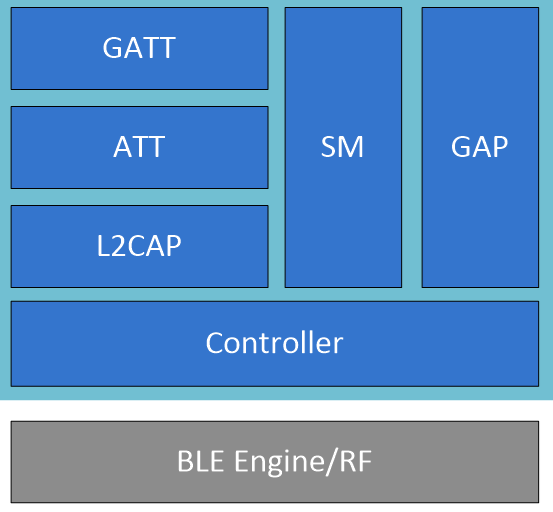
\includegraphics[width=0.5\linewidth]{./img/stack_overview} 

}

\caption{Host 架构}\label{fig:ch0-host-overview}
\end{figure}

Host 任务的伪代码如下:

\begin{Shaded}
\begin{Highlighting}[]
\DataTypeTok{void}\NormalTok{ host_task(}\DataTypeTok{void}\NormalTok{)}
\NormalTok{\{}
\NormalTok{    host_init();}
    \ControlFlowTok{while}\NormalTok{ (true)}
\NormalTok{    \{}
        \ControlFlowTok{if}\NormalTok{ (recv_msg(msg) != }\DecValTok{0}\NormalTok{) }\ControlFlowTok{continue}\NormalTok{;}
\NormalTok{        process_msg(msg);}
\NormalTok{    \}}
\NormalTok{\}}
\end{Highlighting}
\end{Shaded}

也就是说 Host 任务是由各种消息驱动的。这些消息既包括来自 Controller 的事件、ACL 数据,
也包含软件定时器消息和用户发送的消息(\texttt{btstack\_push\_user\_msg})。

\texttt{process\_msg} 的伪代码如下:

\begin{Shaded}
\begin{Highlighting}[]
\DataTypeTok{void}\NormalTok{ process_msg(msg)}
\NormalTok{\{}
    \ControlFlowTok{switch}\NormalTok{ (msg)}
\NormalTok{    \{}
    \ControlFlowTok{case}\NormalTok{ HCI Event:}
\NormalTok{        调用各个回调();}
        \ControlFlowTok{break}\NormalTok{;}
    \ControlFlowTok{case}\NormalTok{ ACL 数据:}
\NormalTok{        调用各个回调();}
        \ControlFlowTok{break}\NormalTok{;}
    \ControlFlowTok{case}\NormalTok{ 软件定时器:}
\NormalTok{        超时处理();}
        \ControlFlowTok{break}\NormalTok{;}
    \ControlFlowTok{case}\NormalTok{ 用户消息:}
\NormalTok{        弹出用户消息事件();}
        \ControlFlowTok{break}\NormalTok{;}
\NormalTok{    \}}
\NormalTok{\}}
\end{Highlighting}
\end{Shaded}

各个模块(包含协议内部模块及 App\footnote{如无特殊说明,本文所说的 App 皆指运行在芯片上的蓝牙程序。})通过注册回调函数以响应这些事件。
有的模块在处理这些消息时又会产生其它的新事件,
为了响应这些新事件可以再向这些模块注册回调函数。也就是说,Host 内部各个模块(以及 App)通过消息、回调函数耦合在一起。
例如:

\begin{itemize}
\item
  \texttt{hci\_add\_event\_handler}

  通过这个函数可以注册一个能够监听所有 HCI 事件的回调;
\item
  \texttt{att\_server\_init}

  向 ATT Server 模块注册用以响应特征读写的回调函数。
\end{itemize}

\hypertarget{ux901aux4fe1ux6a21ux578b}{%
\section{通信模型}\label{ux901aux4fe1ux6a21ux578b}}

通信是指由一地向另一地进行信息的传输与交换,其目的是传输信息、削减另一地的不确定性。对于 BLE 而言,主要有两种通信方式:
一对多的广播、一对一的连接。低功耗蓝牙定义了四种角色:广播发送方称为广播者(Broadcaster),接收方称为观察者(Observer);
连接的发起方称为主角色(新名称为中心角色,Central),接受方称为从角色(新名称为外围角色,Periperhal)。

蓝牙规范定义了广播数据的格式、AD 类型,见图 \ref{fig:ch0-adv-data-format}。如,AD 类型 \(0x09\) 表示设备名称,其后面的 AD 数据域是一个 UTF-8 字符串。
另请参阅``\protect\hyperlink{ch1-adv-data-edit}{广播数据}''一节。

\begin{figure}

{\centering 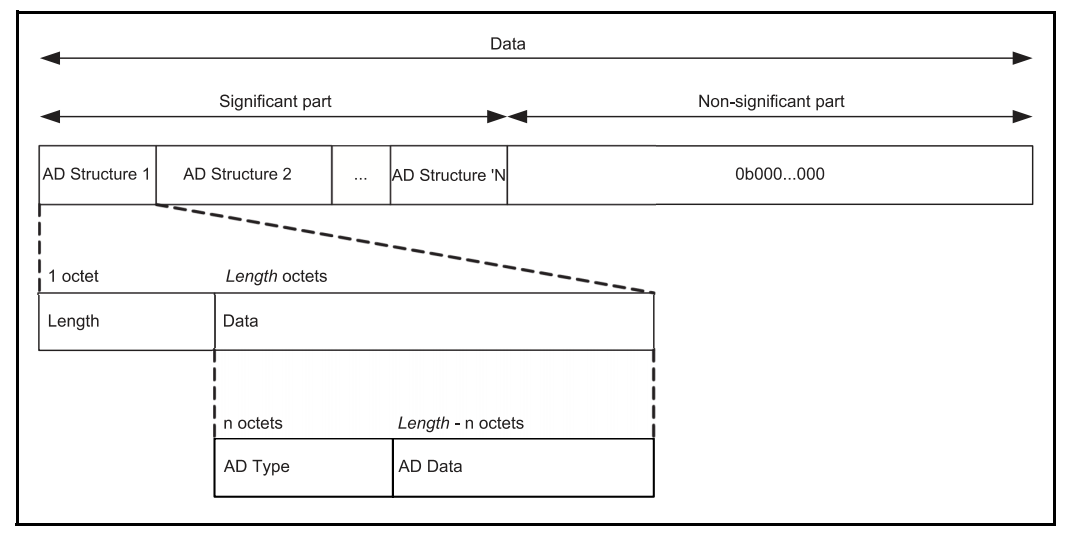
\includegraphics[width=0.8\linewidth]{./img/adv_data_format} 

}

\caption{广播及扫描响应数据包格式}\label{fig:ch0-adv-data-format}
\end{figure}

对于连接模式,低功耗蓝牙定义了特征(Characteristic)和值(Value)这两个概念,进而组织成服务(Service),再由服务组成配置(Profile)。
特征的标识用 UUI​D 标识。客户端发现了服务器支持的服务后,就可以读写特征的值,或者订阅特征\footnote{指示服务器端主动报告特征的值。}。
显然特征不见得支持所有这些操作,因此,蓝牙核心规范又为特征定义了属性(Property)、
描述符(Discriptor)等装饰物,以说明特征所支持的操作、需要的权限。UUID 长度为 \(16\) 字节,为了提高传输效率,BLE 定义了一系列特殊的 UUID,
它们的区别仅在于 2 个字节,另外 \(14\) 个字节相同:

\begin{verbatim}
0x0000xxxx-0000-1000-8000-00805F9B34FB
\end{verbatim}

这两个字节就是所谓的 16-bit UUID,由蓝牙特别兴趣小组公司负责管理、分配\footnote{\url{https://www.bluetooth.com/16-bit-uuids-for-sdos/}}。

\hypertarget{ux56deux8c03ux51fdux6570ux4e8bux4ef6ux5305}{%
\section{回调函数事件包}\label{ux56deux8c03ux51fdux6570ux4e8bux4ef6ux5305}}

协议栈的各种回调函数遵循类似的原型,其输入称为事件包:

\begin{Shaded}
\begin{Highlighting}[]
\KeywordTok{typedef} \DataTypeTok{void}\NormalTok{ (*btstack_packet_handler_t) (}
    \CommentTok{// 事件包类型}
    \DataTypeTok{uint8_t}\NormalTok{ packet_type,}
    \CommentTok{// 关联的信道(一般指蓝牙连接句柄)}
    \DataTypeTok{uint16_t}\NormalTok{ channel,}
    \CommentTok{// 事件包内容}
    \DataTypeTok{const} \DataTypeTok{uint8_t}\NormalTok{ *packet,}
    \CommentTok{// 事件包内容的长度}
    \DataTypeTok{uint16_t}\NormalTok{ size);}
\end{Highlighting}
\end{Shaded}

包类型 \texttt{packet\_type} 的取值如下:

\begin{itemize}
\item
  \texttt{HCI\_EVENT\_PACKET}:HCI 事件包(\textbf{常用})

  这个类型的事件包是个``大杂烩'',多个模块弹出的事件包都会使用这个类型。
\item
  \texttt{HCI\_ACL\_DATA\_PACKET}:Controller 上报的 ACL 数据

  这个类型的事件包只会被通过 \texttt{hci\_register\_acl\_packet\_handler} 注册的 ACL 数据回调函数收到。
\item
  \texttt{HCI\_COMPLETED\_SDU\_PACKET}:来自 LE 信用信道的完整 SDU

  这个类型的事件包只会被通过 \texttt{l2cap\_register\_service} 注册的 L2CAP 服务回调函数收到。
\item
  \texttt{L2CAP\_EVENT\_PACKET}:来自 L2CAP 的事件包

  这个类型的事件包只会被通过 \texttt{l2cap\_add\_event\_handler} 注册的 L2CAP 事件回调函数收到。
\end{itemize}

\hypertarget{ux4e8bux4ef6ux5305ux7684ux89e3ux6790}{%
\section{事件包的解析}\label{ux4e8bux4ef6ux5305ux7684ux89e3ux6790}}

下面只介绍 \texttt{HCI\_EVENT\_PACKET} 事件包的解析,其它几种类型不常用。

首先使用 \texttt{hci\_event\_packet\_get\_type(packet)} 获取事件代码,根据事件代码的不同,后续的处理大不相同。
常用的几种事件代码如下。

\begin{enumerate}
\def\labelenumi{\arabic{enumi}.}
\item
  \texttt{BTSTACK\_EVENT\_STATE}:蓝牙协议栈事件

  一般用于响应协议栈初始化:

\begin{Shaded}
\begin{Highlighting}[]
\ControlFlowTok{if}\NormalTok{ (btstack_event_state_get_state(packet) != HCI_STATE_WORKING)}
    \ControlFlowTok{break}\NormalTok{;}
\CommentTok{// App 初始化}
\end{Highlighting}
\end{Shaded}
\item
  \texttt{HCI\_EVENT\_LE\_META}:BLE 元事件

  这个元事件下辖多个子事件。先通过 \texttt{hci\_event\_le\_meta\_get\_subevent\_code(packet)} 获得子事件代码,然后通过
  \texttt{decode\_hci\_le\_meta\_event(packet,\ sub\_event\_type)} 宏得到子事件的内容。
  \texttt{sub\_event\_type} 为子事件内容对应的数据类型,各字段与蓝牙核心规范里的定义一致\footnote{私有事件(如 HCI\_SUBEVENT\_LE\_VENDOR\_PRO\_CONNECTIONLESS\_IQ\_REPORT)除外。}。

  协议栈的版本及初始化流程导致下列子事件不会出现,只会出现对应的扩展过的、功能更全面的事件:

  \begin{itemize}
  \item
    \texttt{HCI\_SUBEVENT\_LE\_CONNECTION\_COMPLETE}

    改用 \texttt{HCI\_SUBEVENT\_LE\_ENHANCED\_CONNECTION\_COMPLETE}
  \item
    \texttt{HCI\_SUBEVENT\_LE\_ADVERTISING\_REPORT}

    改用 \texttt{HCI\_SUBEVENT\_LE\_EXTENDED\_ADVERTISING\_REPORT}
  \end{itemize}

  协议栈可能报告的子事件及对应的 \texttt{sub\_event\_type} 类型如下:

  \begin{itemize}
  \item
    \texttt{HCI\_SUBEVENT\_LE\_CONNECTION\_UPDATE\_COMPLETE}

    连接参数更新(\texttt{le\_event\_conn\_update\_complete\_t})
  \item
    \texttt{HCI\_SUBEVENT\_LE\_READ\_REMOTE\_USED\_FEATURES\_COMPLETE}

    读取对端特性(\texttt{le\_event\_read\_remote\_feature\_complete\_t})
  \item
    \texttt{HCI\_SUBEVENT\_LE\_LONG\_TERM\_KEY\_REQUEST}

    请求 LTK(\texttt{le\_event\_long\_term\_key\_request\_t})
  \item
    \texttt{HCI\_SUBEVENT\_LE\_REMOTE\_CONNECTION\_PARAMETER\_REQUEST\_COMPLETE}

    远端连接参数请求(\texttt{le\_event\_remote\_conn\_param\_request\_t})
  \item
    \texttt{HCI\_SUBEVENT\_LE\_DATA\_LENGTH\_CHANGE\_EVENT}

    数据包长度改变(\texttt{le\_event\_data\_length\_changed\_t})
  \item
    \texttt{HCI\_SUBEVENT\_LE\_ENHANCED\_CONNECTION\_COMPLETE}

    连接建立(\texttt{le\_event\_create\_conn\_complete\_t})
  \item
    \texttt{HCI\_SUBEVENT\_LE\_DIRECT\_ADVERTISING\_REPORT}

    定向广播报告(\texttt{le\_directed\_adv\_report\_t})
  \item
    \texttt{HCI\_SUBEVENT\_LE\_PHY\_UPDATE\_COMPLETE}

    PHY 更新完成(\texttt{le\_phy\_update\_complete\_t})
  \item
    \texttt{HCI\_SUBEVENT\_LE\_EXTENDED\_ADVERTISING\_REPORT}

    扩展广播报告(\texttt{le\_event\_ext\_adv\_report\_t})
  \item
    \texttt{HCI\_SUBEVENT\_LE\_PERIODIC\_ADVERTISING\_SYNC\_ESTABLISHED}

    周期广播同步建立(\texttt{le\_event\_periodic\_adv\_sync\_established\_t})
  \item
    \texttt{HCI\_SUBEVENT\_LE\_PERIODIC\_ADVERTISING\_REPORT}

    周期广播报告(\texttt{le\_event\_periodic\_adv\_report\_t})
  \item
    \texttt{HCI\_SUBEVENT\_LE\_PERIODIC\_ADVERTISING\_SYNC\_LOST}

    周期广播同步丢失(\texttt{le\_event\_periodic\_adv\_sync\_lost\_t})
  \item
    \texttt{HCI\_SUBEVENT\_LE\_SCAN\_TIMEOUT}

    扫描超时
  \item
    \texttt{HCI\_SUBEVENT\_LE\_ADVERTISING\_SET\_TERMINATED}

    广播停止(\texttt{le\_adv\_seterminated\_t})

    如果是由于广播是由于建立了连接而停止,那么从这个事件里可以得到广播句柄和连接句柄的对应关系。
  \item
    \texttt{HCI\_SUBEVENT\_LE\_SCAN\_REQUEST\_RECEIVED}

    收到扫描请求(\texttt{le\_scan\_req\_received\_t})
  \item
    \texttt{HCI\_SUBEVENT\_LE\_CHANNEL\_SELECTION\_ALGORITHM}

    信道选择算法(\texttt{le\_ch\_sel\_algo\_t})
  \item
    \texttt{HCI\_SUBEVENT\_LE\_CONNECTIONLESS\_IQ\_REPORT}

    无连接 IQ 报告(\texttt{le\_connless\_iq\_report\_t})
  \item
    \texttt{HCI\_SUBEVENT\_LE\_CONNECTION\_IQ\_REPORT}

    有连接 IQ 报告(\texttt{le\_conn\_iq\_report\_t})
  \item
    \texttt{HCI\_SUBEVENT\_LE\_CTE\_REQ\_FAILED}

    CTE 请求失败(\texttt{le\_cte\_req\_failed\_t})
  \item
    \texttt{HCI\_SUBEVENT\_LE\_PRD\_ADV\_SYNC\_TRANSFER\_RCVD}

    周期广播转移请求(\texttt{le\_prd\_adv\_sync\_transfer\_recv\_t})
  \item
    \texttt{HCI\_SUBEVENT\_LE\_REQUEST\_PEER\_SCA}

    对端 SCA 请求完成(\texttt{le\_request\_peer\_sca\_complete\_t})
  \item
    \texttt{HCI\_SUBEVENT\_LE\_PATH\_LOSS\_THRESHOLD}

    路损门限报告(\texttt{le\_path\_loss\_threshold\_t})
  \item
    \texttt{HCI\_SUBEVENT\_LE\_TRANSMIT\_POWER\_REPORTING}

    发射功率报告(\texttt{le\_tx\_power\_reporting\_t})
  \item
    \texttt{HCI\_SUBEVENT\_LE\_SUBRATE\_CHANGE}

    减速模式改变(\texttt{le\_subrate\_change\_t})
  \item
    \texttt{HCI\_SUBEVENT\_LE\_VENDOR\_PRO\_CONNECTIONLESS\_IQ\_REPORT}

    私有无连接 IQ 报告(\texttt{le\_pro\_connless\_iq\_report\_t})
  \end{itemize}
\item
  \texttt{HCI\_EVENT\_DISCONNECTION\_COMPLETE}:连接断开事件

  通过 \texttt{decode\_hci\_event\_disconn\_complete(packet)} 解析事件内容:

\begin{Shaded}
\begin{Highlighting}[]
\KeywordTok{typedef} \KeywordTok{struct}\NormalTok{ event_disconn_complete}
\NormalTok{\{}
    \CommentTok{// 状态码}
    \DataTypeTok{uint8_t}\NormalTok{ status;}
    \CommentTok{// 连接句柄}
    \DataTypeTok{uint16_t}\NormalTok{ conn_handle;}
    \CommentTok{// 原因}
    \DataTypeTok{uint8_t}\NormalTok{ reason;}
\NormalTok{\} event_disconn_complete_t;}
\end{Highlighting}
\end{Shaded}
\item
  \texttt{HCI\_EVENT\_COMMAND\_COMPLETE}:HCI 命令完成事件

  通过 \texttt{hci\_event\_command\_complete\_get\_command\_opcode(packet)} 获得 HCI 命令码。
  通过 \texttt{hci\_event\_command\_complete\_get\_return\_parameters(packet)} 获得 Controller 返回的参数,其中第 1 个字节为命令完成的状态,
  \(0\) 表示没有错误,详见 \protect\hyperlink{ch-ctrl-err-code}{Controller 错误码}。其它参数需要根据命令码做具体分析。
\item
  \texttt{HCI\_EVENT\_COMMAND\_STATUS}:HCI 命令状态事件

  有些 HCI 命令可以立即完成,得到结果,Controller 会上报相应的 \texttt{HCI\_EVENT\_COMMAND\_COMPLETE}。有些 HCI 命令则需要一定时间才能完成,比如发起连接,
  Controller 收到这样的命令后不上报 \texttt{HCI\_EVENT\_COMMAND\_COMPLETE},而是上报 \texttt{HCI\_EVENT\_COMMAND\_STATUS}。

  通过 \texttt{hci\_event\_command\_status\_get\_command\_opcode(packet)} 获得 HCI 命令码。
  通过 \texttt{hci\_event\_command\_status\_get\_status(packet)} 获得状态,\(0\) 表示没有错误,详见 \protect\hyperlink{ch-ctrl-err-code}{Controller 错误码}。
\item
  \texttt{BTSTACK\_EVENT\_USER\_MSG}:来自 \texttt{btstack\_push\_user\_msg} 的用户消息
\end{enumerate}

\hypertarget{ch-ctrl-err-code}{%
\section{Controller 错误码}\label{ch-ctrl-err-code}}

表 \ref{tab:ch0-ctrl-err-code} 列出了 Controller 使用的部分错误码。

\begin{longtable}[]{@{}ll@{}}
\caption{\label{tab:ch0-ctrl-err-code} Controller 错误码}\tabularnewline
\toprule
错误码 & 含义\tabularnewline
\midrule
\endfirsthead
\toprule
错误码 & 含义\tabularnewline
\midrule
\endhead
0x00 & 无错误\tabularnewline
0x01 & 未知的命令\tabularnewline
0x02 & 未知的连接句柄\tabularnewline
0x03 & 硬件错误\tabularnewline
0x05 & 鉴权失败\tabularnewline
0x06 & PIN 或密钥缺失\tabularnewline
0x07 & 超出内存容量\tabularnewline
0x08 & 连接超时\tabularnewline
0x09 & 连接数目达到极限\tabularnewline
0x0B & 连接已存在\tabularnewline
0x0C & 命令不允许\tabularnewline
0x11 & 不支持的特性或参数值\tabularnewline
0x12 & HCI 命令参数错误\tabularnewline
0x13 & 远端用户断开连接\tabularnewline
0x14 & 远端设备因资源紧张断开连接\tabularnewline
0x15 & 远端设备因关机断开连接\tabularnewline
0x16 & 本机断开连接\tabularnewline
0x1A & 不支持的远端或 LMP 特性\tabularnewline
0x1E & 非法的 LMP 或 LL 参数\tabularnewline
0x1F & 未指定的错误\tabularnewline
0x20 & 不支持的 LMP 或 LL 参数\tabularnewline
0x22 & LMP 或 LL 响应超时\tabularnewline
0x23 & LMP 错误(会话冲突)\tabularnewline
0x28 & 时机已过\tabularnewline
0x2E & 不支持信道分类\tabularnewline
0x2F & 安全特性不足\tabularnewline
0x3A & Controller 正忙\tabularnewline
0x3C & 定向广播超时\tabularnewline
0x3D & 因 MIC 错误而断开连接\tabularnewline
0x3E & 连接无法建立\tabularnewline
0x43 & 到达极限\tabularnewline
0xFE & 任务调度失败(私有错误码)\tabularnewline
0xFF & 其它错误(私有错误码)\tabularnewline
\bottomrule
\end{longtable}

\hypertarget{ux767dux540dux5355}{%
\section{白名单}\label{ux767dux540dux5355}}

在广播、扫描或者建立连接时,都可能用到白名单。操作白名单的 API 共有 3 个:

\begin{enumerate}
\def\labelenumi{\arabic{enumi}.}
\item
  \texttt{gap\_clear\_white\_lists}:清空白名单
\item
  \texttt{gap\_add\_whitelist}:添加一个设备地址
\item
  \texttt{gap\_remove\_whitelist}:删除一个设备地址
\end{enumerate}

\hypertarget{ux5f02ux6b65ux7279ux6027}{%
\section{异步特性}\label{ux5f02ux6b65ux7279ux6027}}

Host API 绝大多数都是异步非阻塞操作,比如调用 \texttt{gap\_set\_ext\_adv\_enable()} 并不立即使能广播:这个函数只会给 Controller
发送一条 HCI 消息\footnote{更准确地说,只是把一条 HCI 消息放入消息队列。},Controller 接收消息、完成处理之后才会真正开始广播。

这种异步特性可能使得实现某些功能的代码冗长、零散,开发者可以考虑使用其它语言\footnote{\url{https://ingchips.github.io/blog/2021-01-25-zig-async/}},
或者重新封装 Host API,使其变为同步操作(参考 GATT - 客户端 ``\protect\hyperlink{gatt-client-synced-api}{使用同步版 API}''一节)。

\hypertarget{ux7ebfux7a0bux5b89ux5168ux6027}{%
\section{线程安全性}\label{ux7ebfux7a0bux5b89ux5168ux6027}}

Host 是线程\textbf{不安全}的,除了 \texttt{btstack\_push\_user\_msg} 之外的所有 API 都必须在 Host 任务的上下文内调用。
当其它任务需要调用 Host API 时,必须先通过 \texttt{btstack\_push\_user\_msg} 发送一条消息,再在消息的回调里调用。

\begin{rmdcaution}
开发者在其它任务里直接调用 Host
API,即便发现功能正常,也仅是偶然现象,无法保证总是正常。
\end{rmdcaution}

\hypertarget{ble-ux8bbeux5907ux5730ux5740}{%
\section{BLE 设备地址}\label{ble-ux8bbeux5907ux5730ux5740}}

BLE 设备地址长度为 6 字节,外加 1 个比特表示地址类型。BLE 规范定义了若干种地址类型:

\begin{enumerate}
\def\labelenumi{\arabic{enumi}.}
\item
  公共地址(Public Address,地址类型为 0)

  指从 IEEE 注册机构(IEEE Registration Authority)获得的全球唯一的 EUI-48 地址。
\item
  随机地址(Random Address,地址类型为 1)

  以下几种随机地址类型通过最高的 2 个比特区分。

  \begin{enumerate}
  \def\labelenumii{\arabic{enumii}.}
  \item
    静态设备地址(最高 2 个比特为 0b11)

    可随机生成,可以每次上电后重新生成\footnote{地址改变后,曾与之配对的设备无法自动重连。},但是整个上电周期内不能改变。
  \item
    私有地址

    共有两种私有地址。

    \begin{enumerate}
    \def\labelenumiii{\arabic{enumiii}.}
    \item
      可解析私有地址(最高 2 个比特为 0b01)
    \item
      不可解析私有地址(最高 2 个比特为 0b00)
    \end{enumerate}
  \end{enumerate}
\end{enumerate}

多数情况下四处广播设备的公共地址或者静态地址显然不是一个好主意,使用私有地址可有效地保护隐私。
有了可解析地址的概念后,设备的公共地址、静态地址就从逻辑上变成身份地址(Identity Address)。

\begin{rmdcaution}
\emph{INGCHIPS} 918xx/916xx
系列芯片没有公共地址,只能通过编程配置随机地址。
\end{rmdcaution}

使用蓝牙地址时要注意字节顺序。协议栈遵循下面的基本规律:

\begin{itemize}
\tightlist
\item
  API 使用大端模式
\item
  BLE 元事件使用小端模式\footnote{参照蓝牙核心规范。}
\end{itemize}

使用 \texttt{reverse\_bd\_addr} 可以翻转地址的字节顺序:

\begin{Shaded}
\begin{Highlighting}[]
\DataTypeTok{void}\NormalTok{ reverse_bd_addr(}
    \CommentTok{// 待翻转的地址}
    \DataTypeTok{const} \DataTypeTok{uint8_t}\NormalTok{ *src,}
    \CommentTok{// 输出(不能与 src 相同)}
    \DataTypeTok{uint8_t}\NormalTok{ * dest);}
\end{Highlighting}
\end{Shaded}

\hypertarget{ch-adv}{%
\chapter{GAP - 广播}\label{ch-adv}}

\hypertarget{ux6982ux89c8}{%
\section{概览}\label{ux6982ux89c8}}

支持 4.0 \textasciitilde{} 5.1 规范定义的所有 BLE 广播类型:

\begin{itemize}
\tightlist
\item
  传统广播(Legacy Adv)
\item
  扩展广播(Extended Adv)
\item
  周期广播(Periodic Adv)
\end{itemize}

传统广播的有效载荷最长为 \(31B\),而扩展广播(包括周期广播)每个广播包的有效载荷最长接近 \(255B\),
每个扩展广播又可包含多个广播包(广播包链条),总有效载荷最长达 \(1650B\)。

\hypertarget{ux7c7bux578b}{%
\subsection{类型}\label{ux7c7bux578b}}

广播有几种不同的属性:

\begin{itemize}
\item
  可连接:接受对方发来的连接建立请求
\item
  可扫描:接受对方发来的扫描请求,并回复扫描响应
\item
  定向:只用于可连接广播,只接受特定方发来的连接建立请求
\item
  高占空比(High Duty):以更高的频率\footnote{广播间隔小于 \(3.75ms\)。}重复发送广播数据,常用于实现快速重连(定向可连接广播),
  最长只持续 \(1.28s\)。从 5.0 开始,高占空比广播也可用于不可连接广播。
\end{itemize}

对于传统的扫描响应包,其有效载荷最长同样为 \(31B\);扩展的扫描响应包,其有效载荷最长同样为 \(1650B\)。
开发者可以要求协议栈收到扫描请求时上报事件。

总结起来,传统广播共有 5 种类型,见表 \ref{tab:ch1-legacy-adv-types}。

\begin{longtable}[]{@{}llll@{}}
\caption{\label{tab:ch1-legacy-adv-types} 传统广播类型}\tabularnewline
\toprule
类型 & PDU 类型 & 广播数据 & 扫描响应数据\tabularnewline
\midrule
\endfirsthead
\toprule
类型 & PDU 类型 & 广播数据 & 扫描响应数据\tabularnewline
\midrule
\endhead
非定向可连接可扫描广播 & ADV\_IND & 支持 & 支持\tabularnewline
定向可连接广播(非高占空比) & ADV\_DIRECT\_IND & 不支持 & 不支持\tabularnewline
定向可连接广播(高占空比) & ADV\_DIRECT\_IND & 不支持 & 不支持\tabularnewline
非定向可扫描广播 & ADV\_SCAN\_IND & 支持 & 支持\tabularnewline
非定向不可连接不可扫描广播 & ADV\_NONCONN\_IND & 支持 & 不支持\tabularnewline
\bottomrule
\end{longtable}

\hypertarget{ch1-adv-filter}{%
\subsection{过滤策略}\label{ch1-adv-filter}}

对于可连接或可扫描广播,可以只接受某些设备的连接建立请求或扫描请求,这就是所谓的过滤策略。BLE 定义了 4 种策略:

\begin{Shaded}
\begin{Highlighting}[]
\KeywordTok{typedef} \KeywordTok{enum}\NormalTok{ adv_filter_policy}
\NormalTok{\{}
    \CommentTok{// 接受所有的连接建立请求或扫描请求}
\NormalTok{    ADV_FILTER_ALLOW_ALL    = }\BaseNTok{0x00}\NormalTok{,}
    \CommentTok{// 只接受白名单内的扫描请求,接收所有的连接建立请求}
\NormalTok{    ADV_FILTER_ALLOW_SCAN_WLST_CON_ALL,}
    \CommentTok{// 只接受白名单内的连接建立请求,接收所有的扫描请求}
\NormalTok{    ADV_FILTER_ALLOW_SCAN_ALL_CON_WLST,}
    \CommentTok{// 只接受白名单内的连接建立请求和扫描请求}
\NormalTok{    ADV_FILTER_ALLOW_SCAN_WLST_CON_WLST}
\NormalTok{\} adv_filter_policy_t;}
\end{Highlighting}
\end{Shaded}

\hypertarget{phy}{%
\subsection{PHY}\label{phy}}

对于扩展广播,既需要在主广播信道(37/38/39)上发送少量信息,也需要在其它信道(即辅广播信道)上发送,所以需要分别设置主、
辅广播信道所使用的 PHY,其中主广播信道只能使用 1M、Coded 等两种 PHY,而辅广播信道 3 种 PHY 皆可。

\hypertarget{ux5e7fux64adux96c6}{%
\subsection{广播集}\label{ux5e7fux64adux96c6}}

从 5.0 开始,BLE 支持并发发送多个广播,每个广播称为一个广播集\footnote{在不引起混淆的前提下,本手册混用``广播''、``广播集''这两个名词。},由广播集句柄指示。
每个广播使用各自独立的参数,包括地址、广播类型、PHY、数据等。
开发者可以为广播集指定一个 4 比特长的 SID。

\hypertarget{ux76f8ux5173ux4e8bux4ef6}{%
\subsection{相关事件}\label{ux76f8ux5173ux4e8bux4ef6}}

\begin{itemize}
\item
  \texttt{HCI\_SUBEVENT\_LE\_ADVERTISING\_SET\_TERMINATED}

  一个广播集停止广播时,HCI 回调会收到 \texttt{HCI\_SUBEVENT\_LE\_ADVERTISING\_SET\_TERMINATED} 事件。这个事件的触发条件如下:

  \begin{itemize}
  \tightlist
  \item
    通过 GAP API 停止广播;
  \item
    连接建立;
  \item
    已达到预定的广播时长、次数,自动停止;
  \item
    极端情况:Controller 无法完成任务处理。
  \end{itemize}
\item
  \texttt{HCI\_SUBEVENT\_LE\_SCAN\_REQUEST\_RECEIVED}

  开发者使能扫描请求指示后,HCI 回调会收到 \texttt{HCI\_SUBEVENT\_LE\_SCAN\_REQUEST\_RECEIVED} 事件。
\end{itemize}

\hypertarget{ux4f7fux7528ux8bf4ux660e}{%
\section{使用说明}\label{ux4f7fux7528ux8bf4ux660e}}

\hypertarget{ux914dux7f6eux5e7fux64ad}{%
\subsection{配置广播}\label{ux914dux7f6eux5e7fux64ad}}

主要用到 4 个函数,\texttt{gap\_set\_adv\_set\_random\_addr}、\texttt{gap\_set\_ext\_adv\_para}、\texttt{gap\_set\_ext\_adv\_data} 和 \texttt{gap\_set\_ext\_scan\_response\_data},
分别配置随机地址、参数、广播数据和扫描响应数据。
参数最复杂的函数是 \texttt{gap\_set\_ext\_adv\_para},其原型为:

\begin{Shaded}
\begin{Highlighting}[]
\DataTypeTok{uint8_t}\NormalTok{ gap_set_ext_adv_para(}
    \CommentTok{// 广播集句柄}
    \DataTypeTok{const} \DataTypeTok{uint8_t}\NormalTok{ adv_handle,}
    \CommentTok{// 属性比特组合}
    \DataTypeTok{const}\NormalTok{ adv_event_properties_t properties,}
    \CommentTok{// 广播间隔}
    \DataTypeTok{const} \DataTypeTok{uint32_t}\NormalTok{ interval_min,}
    \DataTypeTok{const} \DataTypeTok{uint32_t}\NormalTok{ interval_max,}
    \CommentTok{// 使用的主广播信道比特组合(0x7 表示使用全部 3 个主广播信道)}
    \DataTypeTok{const}\NormalTok{ adv_channel_bits_t primary_adv_channel_map,}
    \CommentTok{// 使用的地址类型(随机地址来自 gap_set_adv_set_random_addr)}
    \DataTypeTok{const}\NormalTok{ bd_addr_type_t own_addr_type,}
    \CommentTok{// 设置定向广播的对端地址}
    \DataTypeTok{const}\NormalTok{ bd_addr_type_t peer_addr_type,}
    \DataTypeTok{const} \DataTypeTok{uint8_t}\NormalTok{ *peer_addr,}
    \CommentTok{// 过滤策略}
    \DataTypeTok{const}\NormalTok{ adv_filter_policy_t adv_filter_policy,}
    \CommentTok{// 发射功率,单位为 dBm}
    \DataTypeTok{const} \DataTypeTok{int8_t}\NormalTok{ tx_power,}
    \CommentTok{// 主信道 PHY}
    \DataTypeTok{const}\NormalTok{ phy_type_t primary_adv_phy,}
    \CommentTok{// 是否允许跳过部分辅信道的发送(填 0 表示总是发送)}
    \DataTypeTok{const} \DataTypeTok{uint8_t}\NormalTok{ secondary_adv_max_skip,}
    \CommentTok{// 辅信道 PHY}
    \DataTypeTok{const}\NormalTok{ phy_type_t secondary_adv_phy,}
    \CommentTok{// 广播集 SID}
    \DataTypeTok{const} \DataTypeTok{uint8_t}\NormalTok{ sid,}
    \CommentTok{// 使能扫描请求上报}
    \DataTypeTok{const} \DataTypeTok{uint8_t}\NormalTok{ scan_req_notification_enable);}
\end{Highlighting}
\end{Shaded}

其中,\texttt{properties} 为以下比特的组合:

\begin{Shaded}
\begin{Highlighting}[]
\CommentTok{// 可连接广播}
\PreprocessorTok{#define    CONNECTABLE_ADV_BIT       ...}
\CommentTok{// 可扫描广播}
\PreprocessorTok{#define    SCANNABLE_ADV_BIT         ...}
\CommentTok{// 定向广播}
\PreprocessorTok{#define    DIRECT_ADV_BIT            ...}
\CommentTok{// 高频广播}
\PreprocessorTok{#define    HIGH_DUTY_CIR_DIR_ADV_BIT ...}
\CommentTok{// 传统广播}
\PreprocessorTok{#define    LEGACY_PDU_BIT            ...}
\CommentTok{// 匿名广播}
\PreprocessorTok{#define    ANONY_ADV_BIT             ...}
\CommentTok{// 包含发射功率}
\PreprocessorTok{#define    INC_TX_ADV_BIT            ...}
\end{Highlighting}
\end{Shaded}

对于传统广播,比特组合必须符合表 \ref{tab:ch1-legacy-adv-types} 的定义。
对于扩展广播,不能既可连接又可扫描;不支持高占空比广播。
匿名广播中不包含广播者的地址,所以称为``匿名''广播。附加 \texttt{INC\_TX\_ADV\_BIT} 比特后,
广播内自动包含发射功率,比在载荷内通过 AD 项 ``0x0A - «Tx Power Level»''发送开销更小。

\hypertarget{ch1-adv-data-edit}{%
\subsection{广播数据}\label{ch1-adv-data-edit}}

使用 Wizard 里的广播数据编辑器可以方便地编辑数据\footnote{请参阅 SDK 用户手册。}。
广播数据编辑器同时可以生成一些常数,方便开发者编程修改广播数据。
下面的例子把蓝牙地址的最末两个字节填充到设备名称的最后 4 个字符里。

\begin{enumerate}
\def\labelenumi{\arabic{enumi}.}
\item
  用广播数据编辑器生成初始数据(图 \ref{fig:ch0-gen-adv-data}):

  \begin{figure}

   {\centering 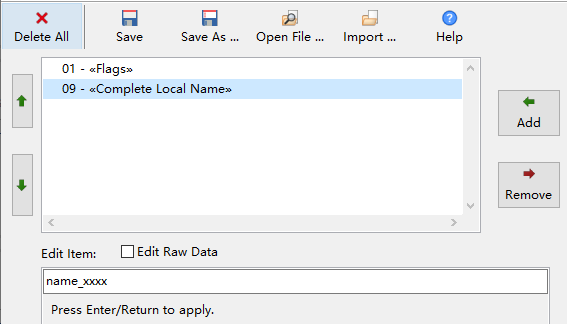
\includegraphics[width=0.6\linewidth]{./img/gen_adv_data} 

   }

   \caption{用广播数据编辑器生成初始数据}\label{fig:ch0-gen-adv-data}
   \end{figure}

\begin{Shaded}
\begin{Highlighting}[]
\CommentTok{// 0x01 - «Flags»}
\DecValTok{2}\NormalTok{, }\BaseNTok{0x01}\NormalTok{,}
\BaseNTok{0x06}\NormalTok{,}

\CommentTok{// 0x09 - «Complete Local Name»: name_xxxx}
\DecValTok{10}\NormalTok{, }\BaseNTok{0x09}\NormalTok{,}
\BaseNTok{0x6E}\NormalTok{, }\BaseNTok{0x61}\NormalTok{, }\BaseNTok{0x6D}\NormalTok{, }\BaseNTok{0x65}\NormalTok{, }\BaseNTok{0x5F}\NormalTok{, }\BaseNTok{0x78}\NormalTok{, }\BaseNTok{0x78}\NormalTok{, }\BaseNTok{0x78}\NormalTok{,}
\BaseNTok{0x78}\NormalTok{,}

\CommentTok{// Total size = 14 bytes}
\end{Highlighting}
\end{Shaded}
\item
  导入广播数据及常数:

\begin{Shaded}
\begin{Highlighting}[]
\DataTypeTok{static} \DataTypeTok{uint8_t}\NormalTok{ adv_data[] = \{}
    \PreprocessorTok{#include }\ImportTok{"../data/advertising.adv"}
\NormalTok{\};}
\CommentTok{// 这个文件里是编辑器生成的常数}
\PreprocessorTok{#include }\ImportTok{"../data/advertising.const"}
\end{Highlighting}
\end{Shaded}
\item
  修改广播名称

\begin{Shaded}
\begin{Highlighting}[]
\DataTypeTok{void}\NormalTok{ assign_name(}\DataTypeTok{const} \DataTypeTok{uint8_t}\NormalTok{ *id_bytes)}
\NormalTok{\{}
    \DataTypeTok{char}\NormalTok{ temp[}\DecValTok{5}\NormalTok{];}
\NormalTok{    sprintf(temp, }\StringTok{"%02X%02X"}\NormalTok{, id_bytes[}\DecValTok{0}\NormalTok{], id_bytes[}\DecValTok{1}\NormalTok{]);}
    \CommentTok{// ADVERTISING_ITEM_OFFSET_COMPLETE_LOCAL_NAME 是编译器自动生成的常数,}
    \CommentTok{// 表示 "name_xxxx" 在整个数据里的偏移位置}
\NormalTok{    memcpy(adv_data + ADVERTISING_ITEM_OFFSET_COMPLETE_LOCAL_NAME + }\DecValTok{5}\NormalTok{,}
\NormalTok{           temp, }\KeywordTok{sizeof}\NormalTok{(temp) - }\DecValTok{1}\NormalTok{);}
\NormalTok{\}}
\CommentTok{// 假设地址存放于 rand_addr}
\NormalTok{assign_name(&rand_addr[}\DecValTok{4}\NormalTok{]);}
\end{Highlighting}
\end{Shaded}
\end{enumerate}

\hypertarget{ux914dux7f6eux5468ux671fux5e7fux64ad}{%
\subsection{配置周期广播}\label{ux914dux7f6eux5468ux671fux5e7fux64ad}}

周期广播总是与一个不可连接、不可扫描的扩展广播绑定。使用 \texttt{gap\_set\_ext\_adv\_para} 设置了扩展广播参数后,
就可以通过 \texttt{gap\_set\_periodic\_adv\_para} 创建相关联的周期广播:

\begin{Shaded}
\begin{Highlighting}[]
\DataTypeTok{uint8_t}\NormalTok{ gap_set_periodic_adv_para(}
  \CommentTok{// 使用同一个广播集句柄}
  \DataTypeTok{const} \DataTypeTok{uint8_t}\NormalTok{ adv_handle,}
  \CommentTok{// 广播周期}
  \DataTypeTok{const} \DataTypeTok{uint16_t}\NormalTok{ interval_min,}
  \DataTypeTok{const} \DataTypeTok{uint16_t}\NormalTok{ interval_max,}
  \CommentTok{// 属性(仅支持 0 或 PERIODIC_ADV_BIT_INC_TX}
  \DataTypeTok{const}\NormalTok{ periodic_adv_properties_t properties);}
\end{Highlighting}
\end{Shaded}

周期广播的数据通过 \texttt{gap\_set\_periodic\_adv\_data} 设置,而不是 \texttt{gap\_set\_ext\_adv\_para}。

\hypertarget{ux8d77ux505cux5e7fux64ad}{%
\subsection{起停广播}\label{ux8d77ux505cux5e7fux64ad}}

通过 \texttt{gap\_set\_ext\_adv\_enable} 控制多个广播集的使能、停止状态。

\begin{Shaded}
\begin{Highlighting}[]
\DataTypeTok{uint8_t}\NormalTok{ gap_set_ext_adv_enable(}
  \CommentTok{// 使能还是停止?}
  \DataTypeTok{const} \DataTypeTok{uint8_t}\NormalTok{ enable,}
  \CommentTok{// 广播集数目}
  \DataTypeTok{const} \DataTypeTok{uint8_t}\NormalTok{ set_number,}
  \CommentTok{// 每个广播集的使能参数}
  \DataTypeTok{const}\NormalTok{ ext_adv_set_en_t *adv_sets);}
\end{Highlighting}
\end{Shaded}

这个函数支持一种快速停止所有广播的用法:\texttt{gap\_set\_ext\_adv\_enable(0,\ 0,\ NULL)}。除此以外,都需要用 \texttt{adv\_sets}
数组表明每个广播集的句柄。

对于使能广播的情况,\texttt{adv\_sets} 使用另外两个参数用来控制广播次数:

\begin{Shaded}
\begin{Highlighting}[]
\KeywordTok{typedef} \KeywordTok{struct}\NormalTok{ ext_adv_set_en}
\NormalTok{\{}
    \DataTypeTok{uint8_t}\NormalTok{ handle;}
    \CommentTok{// 广播持续时间,单位为 10ms。0ms 表示一直广播}
    \DataTypeTok{uint16_t}\NormalTok{ duration;}
    \CommentTok{// 最大广播次数。0 表示一直广播}
    \DataTypeTok{uint8_t}\NormalTok{ max_events;}
\NormalTok{\} ext_adv_set_en_t;}
\end{Highlighting}
\end{Shaded}

当 \texttt{duration} 或 \texttt{max\_events} 条件满足时,广播就会自动停止。

\hypertarget{ux8d77ux505cux5468ux671fux5e7fux64ad}{%
\subsection{起停周期广播}\label{ux8d77ux505cux5468ux671fux5e7fux64ad}}

周期广播需要使用 \texttt{gap\_set\_periodic\_adv\_enable} 控制使能、停止状态:

\begin{Shaded}
\begin{Highlighting}[]
\DataTypeTok{uint8_t}\NormalTok{ gap_set_periodic_adv_enable(}
  \DataTypeTok{const} \DataTypeTok{uint8_t}\NormalTok{ enable,}
  \DataTypeTok{const} \DataTypeTok{uint8_t}\NormalTok{ adv_handle);}
\end{Highlighting}
\end{Shaded}

要``完整''地开启周期广播,需要先通过 \texttt{gap\_set\_ext\_adv\_enable} 使能关联的扩展广播,再用这个 API 使能周期广播。
扩展广播可以独立地关闭\footnote{关闭之后,其它设备无法再与该周期广播建立同步。}。

\hypertarget{ux4e3aux5468ux671fux5e7fux64adux6dfbux52a0-cte}{%
\subsection{为周期广播添加 CTE}\label{ux4e3aux5468ux671fux5e7fux64adux6dfbux52a0-cte}}

参考``\protect\hyperlink{misc-cte-periodic-adv}{基于周期广播的 CTE 接收和发送}''一节。

\hypertarget{ch-scan}{%
\chapter{GAP - 扫描}\label{ch-scan}}

\hypertarget{ux6982ux89c8-1}{%
\section{概览}\label{ux6982ux89c8-1}}

接收广播的过程称为扫描。

\hypertarget{ux95f4ux9694ux4e0eux7a97ux53e3}{%
\subsection{间隔与窗口}\label{ux95f4ux9694ux4e0eux7a97ux53e3}}

接收机实际进行扫描工作的时机受扫描间隔和窗口两个参数控制,其含义如图 \ref{fig:ch2-scan-win-interval} 所示。

\begin{figure}

{\centering 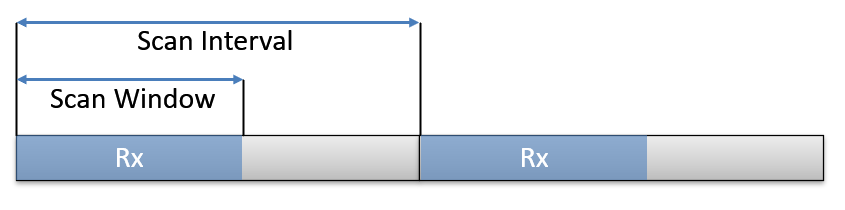
\includegraphics[width=0.7\linewidth]{./img/scan_win_interval} 

}

\caption{扫描间隔与扫描窗口}\label{fig:ch2-scan-win-interval}
\end{figure}

\textbf{注意}:Controller 在执行扫描任务时,遵循最大努力原则,实际真正用于扫描的时机可能并不与两个参数所指定的完全一致。

\hypertarget{ux8fc7ux6ee4ux7b56ux7565}{%
\subsection{过滤策略}\label{ux8fc7ux6ee4ux7b56ux7565}}

与广播的\protect\hyperlink{ch1-adv-filter}{过滤策略}类似,扫描也有几种过滤策略:

\begin{Shaded}
\begin{Highlighting}[]
\KeywordTok{typedef} \KeywordTok{enum}\NormalTok{ scan_filter_policy}
\NormalTok{\{}
    \CommentTok{// 接收所有广播(定向到其它设备的除外)}
\NormalTok{    SCAN_ACCEPT_ALL_EXCEPT_NOT_DIRECTED,}
    \CommentTok{// 只接收来自白名单内的设备的广播(定向到其它设备的除外)}
\NormalTok{    SCAN_ACCEPT_WLIST_EXCEPT_NOT_DIRECTED,}
    \CommentTok{// 接收所有广播(所定向的设备与本设备身份地址不同的除外)}
\NormalTok{    SCAN_ACCEPT_ALL_EXCEPT_IDENTITY_NOT_MATCH,}
    \CommentTok{// 只接收来自白名单内的设备的广播(所定向的设备与本设备身份地址不同的除外)}
\NormalTok{    SCAN_ACCEPT_WLIST_EXCEPT_IDENTITY_NOT_MATCH}
\NormalTok{\} scan_filter_policy_t;}
\end{Highlighting}
\end{Shaded}

\hypertarget{ux4e3bux52a8ux4e0eux88abux52a8}{%
\subsection{主动与被动}\label{ux4e3bux52a8ux4e0eux88abux52a8}}

所谓被动扫描(Passive Scan)指只接收广播数据包,对于可扫描广播也是如此;所谓主动扫描(Active Scan)指除了接收广播数据包之外,
对于可扫描广播会主动发送扫描请求并接收扫描响应包。

\hypertarget{phy-1}{%
\subsection{PHY}\label{phy-1}}

由于扩展广播可在主广播信道使用两种 PHY 发送,相应地,扫描时也需要配置扫描哪种 PHY。

\hypertarget{ux4f7fux7528ux8bf4ux660e-1}{%
\section{使用说明}\label{ux4f7fux7528ux8bf4ux660e-1}}

\hypertarget{ux914dux7f6eux53c2ux6570}{%
\subsection{配置参数}\label{ux914dux7f6eux53c2ux6570}}

在开始扫描之前,需要先通过 \texttt{gap\_set\_random\_device\_address} 为设备配置地址,这个地址用于扫描、发起连接等场景。
使用 \texttt{gap\_set\_ext\_scan\_para} 配置扫描参数:

\begin{Shaded}
\begin{Highlighting}[]
\DataTypeTok{uint8_t}\NormalTok{ gap_set_ext_scan_para(}
  \CommentTok{// 本设备地址类型}
  \DataTypeTok{const}\NormalTok{ bd_addr_type_t own_addr_type,}
  \CommentTok{// 过滤策略}
  \DataTypeTok{const}\NormalTok{ scan_filter_policy_t filter,}
  \CommentTok{// PHY 配置个数}
  \DataTypeTok{const} \DataTypeTok{uint8_t}\NormalTok{ config_num,}
  \CommentTok{// 关于每种 PHY 的参数配置}
  \DataTypeTok{const}\NormalTok{ scan_phy_config_t *configs);}
\end{Highlighting}
\end{Shaded}

每种 PHY 的参数配置如下:

\begin{Shaded}
\begin{Highlighting}[]
\KeywordTok{typedef} \KeywordTok{struct}\NormalTok{ scan_phy_config}
\NormalTok{\{}
    \CommentTok{// PHY}
\NormalTok{    phy_type_t phy;}
    \CommentTok{// 扫描方式:主动或被动}
\NormalTok{    scan_type_t type;}
    \CommentTok{// 扫描间隔,单位是 625us}
    \DataTypeTok{uint16_t}\NormalTok{ interval;}
    \CommentTok{// 扫描窗口,单位是 625us}
    \DataTypeTok{uint16_t}\NormalTok{ window;}
\NormalTok{\} scan_phy_config_t;}
\end{Highlighting}
\end{Shaded}

\hypertarget{ux8d77ux505cux626bux63cf}{%
\subsection{起停扫描}\label{ux8d77ux505cux626bux63cf}}

使用 \texttt{gap\_set\_ext\_scan\_enable} 起停扫描:

\begin{Shaded}
\begin{Highlighting}[]
\DataTypeTok{uint8_t}\NormalTok{ gap_set_ext_scan_enable(}
  \CommentTok{// 开始或者停止扫描}
  \DataTypeTok{const} \DataTypeTok{uint8_t}\NormalTok{ enable,}
  \CommentTok{// 是否对数据做去重处理:0 - 不去重;1 - 去重;}
  \CommentTok{//                       2 - 去重,但是每个周期复位过滤器}
  \DataTypeTok{const} \DataTypeTok{uint8_t}\NormalTok{ filter,}
  \CommentTok{// 持续时间,单位为 10ms}
  \DataTypeTok{const} \DataTypeTok{uint16_t}\NormalTok{ duration,}
  \CommentTok{// 周期,单位为 1.28s}
  \DataTypeTok{const} \DataTypeTok{uint16_t}\NormalTok{ period);}
\end{Highlighting}
\end{Shaded}

\texttt{duration} 和 \texttt{period} 两个参数的目的是实现每个 \texttt{period} 里扫描 \texttt{duration} 长的时间。另有两种特殊情况,从开发者的角度总结如下:

\begin{enumerate}
\def\labelenumi{\arabic{enumi}.}
\tightlist
\item
  持续、一直地扫描:\texttt{duration} 和 \texttt{period} 两个参数皆置为 \(0\)
\item
  只扫描一段时间:\texttt{duration} 置为扫描时长,\texttt{period} 置为 \(0\)
\end{enumerate}

\begin{rmdcaution}
Controller
在做数据去重时遵循最大努力原则,受限于存储空间、处理能力,去重可能失效。
\end{rmdcaution}

\hypertarget{ux5904ux7406ux6570ux636e}{%
\subsection{处理数据}\label{ux5904ux7406ux6570ux636e}}

收到广播包后,HCI 回调函数将收到 \texttt{HCI\_SUBEVENT\_LE\_EXTENDED\_ADVERTISING\_REPORT} 事件。利用 \texttt{decode\_hci\_le\_meta\_event}
宏可将事件转换为 \texttt{le\_ext\_adv\_report\_t} 结构体指针:

\begin{Shaded}
\begin{Highlighting}[]
\DataTypeTok{const}\NormalTok{ le_ext_adv_report_t *report =}
\NormalTok{  decode_hci_le_meta_event(packet, le_meta_event_ext_adv_report_t)->reports;}
\end{Highlighting}
\end{Shaded}

这个结构体的定义如下:

\begin{Shaded}
\begin{Highlighting}[]
\KeywordTok{typedef} \KeywordTok{struct}\NormalTok{ le_ext_adv_report}
\NormalTok{\{}
    \CommentTok{// 事件类型比特位组合}
    \DataTypeTok{uint16_t}\NormalTok{        evt_type;}
    \CommentTok{// 广播者地址类型}
\NormalTok{    bd_addr_type_t  addr_type;}
    \CommentTok{// 广播者地址}
\NormalTok{    bd_addr_t       address;}
    \CommentTok{// 主信道上用的 PHY}
    \DataTypeTok{uint8_t}\NormalTok{         p_phy;}
    \CommentTok{// 辅信道上用的 PHY}
    \DataTypeTok{uint8_t}\NormalTok{         s_phy;}
    \CommentTok{// SID}
    \DataTypeTok{uint8_t}\NormalTok{         sid;}
    \CommentTok{// 发射功率(单位 dBm)}
     \DataTypeTok{int8_t}\NormalTok{         tx_power;}
    \CommentTok{// RSSI (单位 dBm)}
     \DataTypeTok{int8_t}\NormalTok{         rssi;}
    \CommentTok{// 周期广播的间隔(仅对周期广播有效)}
    \DataTypeTok{uint16_t}\NormalTok{        prd_adv_interval;}
    \CommentTok{// 定向广播的目的地址类型}
\NormalTok{    bd_addr_type_t  direct_addr_type;}
    \CommentTok{// 定向广播的目的地址}
\NormalTok{    bd_addr_t       direct_addr;}
    \CommentTok{// 广播数据长度}
    \DataTypeTok{uint8_t}\NormalTok{         data_len;}
    \CommentTok{// 广播数据}
    \DataTypeTok{uint8_t}\NormalTok{         data[}\DecValTok{0}\NormalTok{];}
\NormalTok{\} le_ext_adv_report_t;}
\end{Highlighting}
\end{Shaded}

\hypertarget{ux4e0eux5468ux671fux5e7fux64adux540cux6b65}{%
\subsection{与周期广播同步}\label{ux4e0eux5468ux671fux5e7fux64adux540cux6b65}}

发现周期广播后,可以通过 \texttt{gap\_periodic\_adv\_create\_sync} 与周期广播同步\footnote{即周期性地接收周期广播。}:

\begin{Shaded}
\begin{Highlighting}[]
\DataTypeTok{uint8_t}\NormalTok{ gap_periodic_adv_create_sync(}
  \CommentTok{// 过滤策略:目标地址来自白名单还是参数}
  \DataTypeTok{const}\NormalTok{ periodic_adv_filter_policy_t filter_policy,}
  \CommentTok{// SID}
  \DataTypeTok{const} \DataTypeTok{uint8_t}\NormalTok{ adv_sid,}
  \CommentTok{// 目标地址类型}
  \DataTypeTok{const}\NormalTok{ bd_addr_type_t addr_type,}
  \CommentTok{// 目标地址}
  \DataTypeTok{const} \DataTypeTok{uint8_t}\NormalTok{ *addr,}
  \CommentTok{// 成功接收一次之后,可跳过的数目}
  \DataTypeTok{const} \DataTypeTok{uint16_t}\NormalTok{ skip,}
  \CommentTok{// 同步超时(单位 100ms)}
  \DataTypeTok{const} \DataTypeTok{uint16_t}\NormalTok{ sync_timeout,}
  \CommentTok{// 周期广播里的 CTE 类型(如果存在)}
  \DataTypeTok{const} \DataTypeTok{uint8_t}\NormalTok{ sync_cte_type}
\NormalTok{);}
\end{Highlighting}
\end{Shaded}

成功建立同步后,HCI 回调会收到 \texttt{HCI\_SUBEVENT\_LE\_PERIODIC\_ADVERTISING\_SYNC\_ESTABLISHED} 事件。接收到的周期广播通过
\texttt{HCI\_SUBEVENT\_LE\_PERIODIC\_ADVERTISING\_REPORT} 事件上报,其内容与 \texttt{le\_ext\_adv\_report\_t} 类似。

周期广播的接收可参考 SDK \emph{Periodic Scanner}。

\hypertarget{ch-conn}{%
\chapter{GAP - 连接}\label{ch-conn}}

\hypertarget{ux6982ux89c8-2}{%
\section{概览}\label{ux6982ux89c8-2}}

连接管理功能也由 GAP 模块提供,包含建立连接、断开连接、读取对端版本、减速模式、功率控制等。

\hypertarget{ux4f7fux7528ux8bf4ux660e-2}{%
\section{使用说明}\label{ux4f7fux7528ux8bf4ux660e-2}}

\hypertarget{ux5efaux7acbux8fdeux63a5}{%
\subsection{建立连接}\label{ux5efaux7acbux8fdeux63a5}}

建立连接的过程与主动扫描有相似之处:持续尝试接收某种类型的广播,主动发出一个请求。所以,蓝牙协议规定不要并发地执行这两项任务:
建立连接前要先停止扫描,反之亦然。

在建立连接之前,需要先通过 \texttt{gap\_set\_random\_device\_address} 为设备配置地址,这个地址用于扫描、发起连接等场景。
通过 \texttt{gap\_ext\_create\_connection} 建立连接。所连接的目标可以是一个特定的地址,也可以是白名单中的任意一个地址\footnote{需要连接多个设备,使用白名单方式效率更高。}。

\begin{Shaded}
\begin{Highlighting}[]
\DataTypeTok{uint8_t}\NormalTok{ gap_ext_create_connection(}
  \CommentTok{// 过滤策略:目标地址来自参数还是白名单?}
  \DataTypeTok{const}\NormalTok{ initiating_filter_policy_t filter_policy,}
  \CommentTok{// 本设备地址类型}
  \DataTypeTok{const}\NormalTok{ bd_addr_type_t own_addr_type,}
  \CommentTok{// 目标地址来自参数时,指定目标地址类型}
  \DataTypeTok{const}\NormalTok{ bd_addr_type_t peer_addr_type,}
  \CommentTok{// 目标地址来自参数时,指定目标地址}
  \DataTypeTok{const} \DataTypeTok{uint8_t}\NormalTok{ *peer_addr,}
  \CommentTok{// 主广播信道的配置个数}
  \DataTypeTok{const} \DataTypeTok{uint8_t}\NormalTok{ initiating_phy_num,}
  \CommentTok{// 主广播信道的配置}
  \DataTypeTok{const}\NormalTok{ initiating_phy_config_t *phy_configs);}
\end{Highlighting}
\end{Shaded}

主广播信道的配置 \texttt{initiating\_phy\_config\_t} 指定了每种主广播信道 PHY 的扫描参数(此部分与扫描参数 \texttt{scan\_phy\_config\_t} 相同)及连接参数:

\begin{Shaded}
\begin{Highlighting}[]
\KeywordTok{typedef} \KeywordTok{struct}\NormalTok{ \{}
    \CommentTok{// 同 scan_phy_config_t}
    \DataTypeTok{uint16_t}\NormalTok{ scan_int;}
    \DataTypeTok{uint16_t}\NormalTok{ scan_win;}
    \CommentTok{// 最小连接间隔,单位 1.25ms}
    \DataTypeTok{uint16_t}\NormalTok{ interval_min;}
    \CommentTok{// 最大连接间隔,单位 1.25ms}
    \DataTypeTok{uint16_t}\NormalTok{ interval_max;}
    \CommentTok{// 从机延迟(即允许从机跳过多少个连接间隔)}
    \DataTypeTok{uint16_t}\NormalTok{ latency;}
    \CommentTok{// LE 链路超时时间,单位 10ms}
    \DataTypeTok{uint16_t}\NormalTok{ supervision_timeout;}
    \CommentTok{// 关于每个连接间隔内连接事件长度的提示信息,单位 0.625ms}
    \DataTypeTok{uint16_t}\NormalTok{ min_ce_len;}
    \DataTypeTok{uint16_t}\NormalTok{ max_ce_len;}
\NormalTok{\} conn_para_t;}

\KeywordTok{typedef} \KeywordTok{struct}\NormalTok{ initiating_phy_config}
\NormalTok{\{}
\NormalTok{    phy_type_t phy;}
\NormalTok{    conn_para_t conn_param;}
\NormalTok{\} initiating_phy_config_t;}
\end{Highlighting}
\end{Shaded}

关于每个连接间隔内连接事件长度的提示信息(\texttt{min\_ce\_len} 和 \texttt{max\_ce\_len})不会被传递给从端。Controller 可以借助这个信息更好地调度多种任务。
从端 App 可调用 LL API \texttt{ll\_hint\_on\_ce\_len}\footnote{参考 《Controller API Reference》。} 将提示信息告知 Controller。

收到对应的 \texttt{HCI\_EVENT\_COMMAND\_STATUS} 事件,并且 \texttt{status} 为 \(0\),标志着开始执行连接建立任务。
\texttt{HCI\_SUBEVENT\_LE\_ENHANCED\_CONNECTION\_COMPLETE} 事件标志着连接建立任务的结束。

\begin{rmdcaution}
复杂应用(如多种蓝牙任务并发)中,务必响应
\texttt{HCI\_EVENT\_COMMAND\_STATUS} 事件检查建立连接命令是否出错。
\end{rmdcaution}

\hypertarget{ux53d6ux6d88ux8fdeux63a5}{%
\subsection{取消连接}\label{ux53d6ux6d88ux8fdeux63a5}}

建立连接需要一定的时间,如果决定不再继续等待,可以通过 \texttt{gap\_create\_connection\_cancel} 取消连接建立任务。
任务取消后,同样会上报 \texttt{HCI\_SUBEVENT\_LE\_ENHANCED\_CONNECTION\_COMPLETE} 事件,其中的 \texttt{status} 为 \(0x02\)
(未知的连接句柄)。

\hypertarget{ux83b7ux53d6ux5bf9ux7aefux7248ux672c}{%
\subsection{获取对端版本}\label{ux83b7ux53d6ux5bf9ux7aefux7248ux672c}}

通过 \texttt{gap\_read\_remote\_info} 可以读取对端协议栈版本。获得版本信息后 Controller 上报 \texttt{HCI\_EVENT\_READ\_REMOTE\_VERSION\_INFORMATION\_COMPLETE}
事件。版本的解析方法可参考 SDK \emph{UART GATT Console}。

\hypertarget{ux83b7ux53d6ux5bf9ux7aefux7279ux6027}{%
\subsection{获取对端特性}\label{ux83b7ux53d6ux5bf9ux7aefux7279ux6027}}

通过 \texttt{gap\_read\_remote\_used\_features} 可以读取对端支持的 BLE 特性。获得特性信息后 Controller 上报 \texttt{HCI\_SUBEVENT\_LE\_READ\_REMOTE\_USED\_FEATURES\_COMPLETE}
这个子事件。特性的解析方法可参考 SDK \emph{UART GATT Console}。

\hypertarget{ux8bbeux7f6e-phy}{%
\subsection{设置 PHY}\label{ux8bbeux7f6e-phy}}

通过 \texttt{gap\_set\_phy} 可以设置偏好的 PHY。经过与对方的协商生效后,Controller 上报 \texttt{HCI\_SUBEVENT\_LE\_PHY\_UPDATE\_COMPLETE} 事件。

\texttt{gap\_set\_phy} 参数详解:

\begin{Shaded}
\begin{Highlighting}[]
\DataTypeTok{uint8_t}\NormalTok{ gap_set_phy(}
  \CommentTok{// 连接句柄}
  \DataTypeTok{const} \DataTypeTok{uint16_t}\NormalTok{ con_handle,}
  \CommentTok{// 置起比特 0 表示在发送方向无偏好}
  \CommentTok{// 置起比特 1 表示在接收方向无偏好}
  \CommentTok{// 其它比特保留}
  \DataTypeTok{const} \DataTypeTok{uint8_t}\NormalTok{ all_phys,}
  \CommentTok{// 发送方向上的 PHY 偏好(比特 0 为 0 有效)}
  \DataTypeTok{const}\NormalTok{ phy_bittypes_t tx_phys,}
  \CommentTok{// 接收方向上的 PHY 偏好(比特 1 为 0 有效)}
  \DataTypeTok{const}\NormalTok{ phy_bittypes_t rx_phys,}
  \CommentTok{// PHY 的其它选项}
  \DataTypeTok{const}\NormalTok{ phy_option_t phy_opt);}
\end{Highlighting}
\end{Shaded}

PHY 偏好 \texttt{phy\_bittypes\_t} 是几个比特的组合:

\begin{longtable}[]{@{}ll@{}}
\caption{\label{tab:ch2-phy-bit-types} PHY 比特组合}\tabularnewline
\toprule
比特序号 & 含义\tabularnewline
\midrule
\endfirsthead
\toprule
比特序号 & 含义\tabularnewline
\midrule
\endhead
0 & 1M PHY\tabularnewline
1 & 2M PHY\tabularnewline
2 & Coded PHY\tabularnewline
\bottomrule
\end{longtable}

\texttt{phy\_option\_t} 目前用来指示 Coded PHY 为 S2 还是 S8。

\hypertarget{ux66f4ux65b0ux8fdeux63a5ux53c2ux6570}{%
\subsection{更新连接参数}\label{ux66f4ux65b0ux8fdeux63a5ux53c2ux6570}}

连接中的主角色通过 \texttt{gap\_update\_connection\_parameters} 可以更新连接参数\footnote{从角色使用 \texttt{l2cap\_request\_connection\_parameter\_update} 请求更新。}:

\begin{Shaded}
\begin{Highlighting}[]
\DataTypeTok{int}\NormalTok{ gap_update_connection_parameters(}
  \CommentTok{// 连接句柄}
\NormalTok{  hci_con_handle_t con_handle,}
  \CommentTok{// 建议的最小连接间隔(单位 1.25ms)}
  \DataTypeTok{uint16_t}\NormalTok{ conn_interval_min,}
  \CommentTok{// 建议的最大连接间隔(单位 1.25ms)}
  \DataTypeTok{uint16_t}\NormalTok{ conn_interval_max,}
  \CommentTok{// 建议的从机延迟}
  \DataTypeTok{uint16_t}\NormalTok{ conn_latency,}
  \CommentTok{// 建议的超时时间(单位 10ms)}
  \DataTypeTok{uint16_t}\NormalTok{ supervision_timeout,}
  \CommentTok{// 关于每个连接间隔内连接事件长度的提示信息,单位 0.625ms}
  \DataTypeTok{uint16_t}\NormalTok{ min_ce_len,}
  \DataTypeTok{uint16_t}\NormalTok{ max_ce_len);}
\end{Highlighting}
\end{Shaded}

事件 \texttt{HCI\_SUBEVENT\_LE\_CONNECTION\_UPDATE\_COMPLETE} 标志着参数更新完成。

\hypertarget{ux51cfux901fux6a21ux5f0f}{%
\subsection{减速模式}\label{ux51cfux901fux6a21ux5f0f}}

减速模式的使用方法可参考 SDK \emph{UART GATT Console}。

\hypertarget{ux529fux7387ux63a7ux5236}{%
\subsection{功率控制}\label{ux529fux7387ux63a7ux5236}}

功率控制的使用方法可参考 SDK \emph{UART GATT Console}。

\hypertarget{ch-gatt-server}{%
\chapter{GATT - 服务器}\label{ch-gatt-server}}

\hypertarget{ux6982ux89c8-3}{%
\section{概览}\label{ux6982ux89c8-3}}

GATT 服务器\footnote{在不引起混淆的前提下,本手册混用 ATT 服务器、GATT 服务器,代码里也用 \texttt{att\_server} 代指 \texttt{gatt\_server}。}为客户端提供服务。
协议栈支持多个连接,每个连接的配置(Profile)可以独立设置。
需要注意,GATT 服务器和客户端这两个角色与主、从两个角色没有任何关联:一个连接的主角色既可以充当 GATT 的客户端,也可以充当服务器,
还可以两种角色一起扮演;一个连接的从角色也是如此。

要使用 GATT 服务器,开放者需要做三件事\footnote{事实上,这几件事已由 Wizard 工具代劳。}:

\begin{enumerate}
\def\labelenumi{\arabic{enumi}.}
\item
  初试化:设置事件回调

\begin{Shaded}
\begin{Highlighting}[]
\DataTypeTok{void}\NormalTok{ att_server_register_packet_handler(}
\NormalTok{  btstack_packet_handler_t handler);}
\end{Highlighting}
\end{Shaded}
\item
  初始化:提供调写回调函数

\begin{Shaded}
\begin{Highlighting}[]
\DataTypeTok{void}\NormalTok{ att_server_init(}
  \CommentTok{// 特征的读回调}
\NormalTok{  att_read_callback_t read_callback,}
  \CommentTok{// 特征的写回调}
\NormalTok{  att_write_callback_t write_callback);}
\end{Highlighting}
\end{Shaded}

  读回调的类型如下:

\begin{Shaded}
\begin{Highlighting}[]
\KeywordTok{typedef} \DataTypeTok{uint16_t}\NormalTok{ (*att_read_callback_t)(}
  \CommentTok{// 连接句柄}
\NormalTok{  hci_con_handle_t con_handle,}
  \CommentTok{// 特征句柄}
  \DataTypeTok{uint16_t}\NormalTok{ attribute_handle,}
  \CommentTok{// 数据偏移}
  \DataTypeTok{uint16_t}\NormalTok{ offset,}
  \CommentTok{// 缓存}
  \DataTypeTok{uint8_t}\NormalTok{ *buffer,}
  \CommentTok{// 缓存的大小}
  \DataTypeTok{uint16_t}\NormalTok{ buffer_size);}
\end{Highlighting}
\end{Shaded}

  写回调的类型如下:

\begin{Shaded}
\begin{Highlighting}[]
\KeywordTok{typedef} \DataTypeTok{int}\NormalTok{ (*att_write_callback_t)(}
  \CommentTok{// 连接句柄}
\NormalTok{  hci_con_handle_t con_handle,}
  \CommentTok{// 特征句柄}
  \DataTypeTok{uint16_t}\NormalTok{ attribute_handle,}
  \CommentTok{// 会话模式}
  \DataTypeTok{uint16_t}\NormalTok{ transaction_mode,}
  \CommentTok{// 数据偏移}
  \DataTypeTok{uint16_t}\NormalTok{ offset,}
  \CommentTok{// 缓存}
  \DataTypeTok{const} \DataTypeTok{uint8_t}\NormalTok{ *buffer,}
  \CommentTok{// 缓存的大小}
  \DataTypeTok{uint16_t}\NormalTok{ buffer_size);}
\end{Highlighting}
\end{Shaded}

  将 \texttt{con\_handle} 和 \texttt{attribute\_handle} 组合到一起,回调函数就可以确定是在访问哪个 Profile 里的哪个特征。
  对于长度超过\((ATT\_MTU - 3)\)的长值,BLE 支持分块读写模式,相应地,两个回调函数都有一个 \texttt{offset} 参数。

  关于会话模式 \texttt{transaction\_mode} 的说明见后文。
\item
  适时提供 Profile 数据

\begin{Shaded}
\begin{Highlighting}[]
\DataTypeTok{void}\NormalTok{ att_set_db(}
  \CommentTok{// 要关联的句柄}
\NormalTok{  hci_con_handle_t con_handle,}
  \CommentTok{// Profile 数据库}
  \DataTypeTok{const} \DataTypeTok{uint8_t}\NormalTok{ *db);}
\end{Highlighting}
\end{Shaded}
\end{enumerate}

协议栈内的 GATT 服务器可以通过 2 种方式获得特征的值,然后传输到客户端:

\begin{enumerate}
\def\labelenumi{\arabic{enumi}.}
\item
  保存在 Profile 数据库内部的值

  这种方式适用于值不改变的情况,服务器可能自动将值传输到客户端,不需要开发者参与。
\item
  借助回调函数 \texttt{att\_read\_callback\_t}

  这种方式适用于值动态改变的情况。
  每当客户端读取值时,协议栈会立即调用回调函数,且 \texttt{buffer} 为 \texttt{NULL}。
  这一次调用是为了获取数值长度。回调函数的处理流程又可以分为两种情况:

  \begin{itemize}
  \item
    如果 App 可以立即准备好数据,那么直接返回数值的\textbf{总长};

    之后,协议栈准备内存空间并立即再次调用函数,此时 \texttt{buffer} 参数非 \texttt{NULL},
    回调函数将数据写入 \texttt{buffer} 所指向的内存,读取完成;
  \item
    如果 App 无法立即准备好数据,那么返回 \texttt{ATT\_DEFERRED\_READ} 进入延迟读取模式;

    待数据就绪之后,App 调用 \texttt{att\_server\_deferred\_read\_response} 将数据传给协议栈,读取完成。
  \end{itemize}
\end{enumerate}

每个特性具有若干属性,见表 \ref{tab:ch3-char-properties}。

\begin{longtable}[]{@{}ll@{}}
\caption{\label{tab:ch3-char-properties} 特征的属性}\tabularnewline
\toprule
属性 & 说明\tabularnewline
\midrule
\endfirsthead
\toprule
属性 & 说明\tabularnewline
\midrule
\endhead
ATT\_PROPERTY\_BROADCAST & 允许广播该特性的值\tabularnewline
ATT\_PROPERTY\_READ & 允许读取\tabularnewline
ATT\_PROPERTY\_WRITE\_WITHOUT\_RESPONSE & 允许无响应写入\tabularnewline
ATT\_PROPERTY\_WRITE & 允许(有响应的)写入\tabularnewline
ATT\_PROPERTY\_NOTIFY & 允许通知(Notification)\tabularnewline
ATT\_PROPERTY\_INDICATE & 允许指示(Indication)\tabularnewline
ATT\_PROPERTY\_AUTHENTICATED\_SIGNED\_WRITE & 允许带签名的写入\tabularnewline
ATT\_PROPERTY\_EXTENDED\_PROPERTIES & 支持扩展属性\tabularnewline
ATT\_PROPERTY\_DYNAMIC & 为动态特性(即需要使用回调函数)\tabularnewline
\bottomrule
\end{longtable}

其中 \texttt{DYNAMIC} 为协议栈自定义的属性,只有加上了这个属性,对特性的读写操作才会交由回调函数处理。对于支持写入的特征,
由于总是需要通过回调函数处理,必须加上此属性。

对于支持通知(Notification)和/或指示(Indication)的特征,必须带有 Client Characteristic Configuration
描述符(常被简称为 CCCD):

\begin{itemize}
\tightlist
\item
  将 \texttt{GATT\_CLIENT\_CHARACTERISTICS\_CONFIGURATION\_NOTIFICATION} 写入 CCCD 就可以使能通知,
\item
  将 \texttt{GATT\_CLIENT\_CHARACTERISTICS\_CONFIGURATION\_INDICATION} 写入 CCCD 就可以使能指示,
\item
  将 \texttt{GATT\_CLIENT\_CHARACTERISTICS\_CONFIGURATION\_NONE} 写入 CCCD 就可以关闭通知和指示。
\end{itemize}

通知相当于无响应的上报,而指示相当于有响应的上报。

\hypertarget{ux4f7fux7528ux8bf4ux660e-3}{%
\section{使用说明}\label{ux4f7fux7528ux8bf4ux660e-3}}

\hypertarget{profile-ux6570ux636e}{%
\subsection{Profile 数据}\label{profile-ux6570ux636e}}

Profile 数据\footnote{在手册、工具、代码的不同位置可能使用了不同的名词,如 Profile 数据库、GATT 数据库、GATT 数据等。} 使用了协议栈自定义的数据结构。
开发者不需要了解这个数据结构的定义,而是借助图形化工具或者编程地生成。

\begin{enumerate}
\def\labelenumi{\arabic{enumi}.}
\item
  使用图形化的 Profile 编辑器。

  请参考 《SDK 用户手册》。
\item
  使用 \texttt{att\_db\_util} 模块。

  调用 \texttt{att\_db\_util\_init} 告知 Profile 数据的存储空间。
  调用 \texttt{att\_db\_util\_add\_service\_uuid??} 添加服务,然后通过 \texttt{att\_db\_util\_add\_characteristic\_uuid??} 添加若干特性。
  重复上述步骤可以添加多个服务。最后调用 \texttt{att\_db\_util\_get\_size} 查看整个 Profile 数据的大小,相应调整存储空间的大小,再重新编译程序。

  上面的 \texttt{.....\_uuid??} 函数都包含 \texttt{uuid16} 和 \texttt{uuid128} 等两种形式,分别对应 16-bit 的简短 UUID 和 16 字节的完整 UUID。

  \texttt{att\_db\_util\_add\_characteristic\_uuid??} 函数返回的是特性的值的句柄。
  调用 \texttt{att\_db\_util\_add\_characteristic\_uuid??} 时需要注意根据情况添加 \texttt{ATT\_PROPERTY\_DYNAMIC} 属性。
  对于带有 \texttt{ATT\_PROPERTY\_NOTIFY} 和/或 \texttt{ATT\_PROPERTY\_INDICATE} 属性的特性,\texttt{att\_db\_util\_add\_characteristic\_uuid??} 函数会自动添加 CCCD。
  设特性的值句柄为 \(N\),那么 CCCD 的句柄为 \(N + 1\)。
\end{enumerate}

\hypertarget{ux5b9eux73b0ux8bfbux56deux8c03}{%
\subsection{实现读回调}\label{ux5b9eux73b0ux8bfbux56deux8c03}}

一个典型的读回调函数大概是这种样子:

\begin{Shaded}
\begin{Highlighting}[]
\DataTypeTok{static} \DataTypeTok{uint16_t}\NormalTok{ att_read_callback(hci_con_handle_t connection_handle,}
  \DataTypeTok{uint16_t}\NormalTok{ att_handle, }\DataTypeTok{uint16_t}\NormalTok{ offset,}
  \DataTypeTok{uint8_t}\NormalTok{ * buffer, }\DataTypeTok{uint16_t}\NormalTok{ buffer_size)}
\NormalTok{\{}
    \ControlFlowTok{switch}\NormalTok{ (att_handle)}
\NormalTok{    \{}
    \ControlFlowTok{case}\NormalTok{ HANDLE_0:}
        \ControlFlowTok{if}\NormalTok{ (buffer)}
\NormalTok{        \{}
\NormalTok{            memcpy(buffer, ...)}
            \ControlFlowTok{return}\NormalTok{ buffer_size;}
\NormalTok{        \}}
        \ControlFlowTok{else}
            \ControlFlowTok{return}\NormalTok{ size of value;}
    \CommentTok{//...}
    \ControlFlowTok{default}\NormalTok{:}
        \ControlFlowTok{return} \DecValTok{0}\NormalTok{;}
\NormalTok{    \}}
\NormalTok{\}}
\end{Highlighting}
\end{Shaded}

延迟读取的情况:

\begin{Shaded}
\begin{Highlighting}[]
\DataTypeTok{static} \DataTypeTok{uint16_t}\NormalTok{ att_read_callback(hci_con_handle_t connection_handle,}
  \DataTypeTok{uint16_t}\NormalTok{ att_handle, }\DataTypeTok{uint16_t}\NormalTok{ offset,}
  \DataTypeTok{uint8_t}\NormalTok{ * buffer, }\DataTypeTok{uint16_t}\NormalTok{ buffer_size)}
\NormalTok{\{}
    \ControlFlowTok{switch}\NormalTok{ (att_handle)}
\NormalTok{    \{}
    \ControlFlowTok{case}\NormalTok{ HANDLE_0:}
        \CommentTok{//...}
        \ControlFlowTok{return}\NormalTok{ ATT_DEFERRED_READ;}
    \CommentTok{//...}
    \ControlFlowTok{default}\NormalTok{:}
        \ControlFlowTok{return} \DecValTok{0}\NormalTok{;}
\NormalTok{    \}}
\NormalTok{\}}
\end{Highlighting}
\end{Shaded}

延迟读取的数据通过 \texttt{att\_server\_deferred\_read\_response} 传递给协议栈:

\begin{Shaded}
\begin{Highlighting}[]
\DataTypeTok{int}\NormalTok{ att_server_deferred_read_response(}
  \CommentTok{// 连接句柄}
\NormalTok{  hci_con_handle_t con_handle,}
  \CommentTok{// 特征句柄}
  \DataTypeTok{uint16_t}\NormalTok{ attribute_handle,}
  \CommentTok{// 指向值的指针}
  \DataTypeTok{const} \DataTypeTok{uint8_t}\NormalTok{ *value,}
  \CommentTok{// 值的长度}
  \DataTypeTok{uint16_t}\NormalTok{ value_len);}
\end{Highlighting}
\end{Shaded}

SDK \emph{GATT Relay} 演示了延迟读取的具体用法。

\hypertarget{ux5b9eux73b0ux5199ux56deux8c03}{%
\subsection{实现写回调}\label{ux5b9eux73b0ux5199ux56deux8c03}}

当写特性时,可能触发服务器执行某个动作。BLE 为了精度控制动作的执行引入了会话\footnote{协议栈里称为``会话'',规范里称为``队列''。}概念:
一个会话包含对 1 个或多个特性的写入,最后是一个显式的``执行''命令通知服务器开始执行。此外还有一个``取消''命令,通知服务器会话不要执行动作、直接终止。相应地,
写回调的会话模式 \texttt{transaction\_mode} 参数包含四种值:

\begin{Shaded}
\begin{Highlighting}[]
\CommentTok{// 无会话的普通写入}
\PreprocessorTok{#define ATT_TRANSACTION_MODE_NONE      ...}
\CommentTok{// 带会话的写入}
\PreprocessorTok{#define ATT_TRANSACTION_MODE_ACTIVE    ...}
\CommentTok{// 执行}
\PreprocessorTok{#define ATT_TRANSACTION_MODE_EXECUTE   ...}
\CommentTok{// 取消}
\PreprocessorTok{#define ATT_TRANSACTION_MODE_CANCEL    ...}
\end{Highlighting}
\end{Shaded}

对于 \texttt{NONE} 和 \texttt{ACTIVE} 两种模式,都会传入要写入的数据,而 \texttt{EXECUTE} 和 \texttt{CANCEL} 则既不会传入特征句柄,也不传入数据,
也就是说这两个命令只关联到连接,施加于整个服务器,而不针对某个特征。

一个典型的写回调函数大概是这种样子:

\begin{Shaded}
\begin{Highlighting}[]
\DataTypeTok{static} \DataTypeTok{int}\NormalTok{ att_write_callback(}
\NormalTok{  hci_con_handle_t connection_handle, }\DataTypeTok{uint16_t}\NormalTok{ att_handle,}
  \DataTypeTok{uint16_t}\NormalTok{ transaction_mode,}
  \DataTypeTok{uint16_t}\NormalTok{ offset, }\DataTypeTok{const} \DataTypeTok{uint8_t}\NormalTok{ *buffer, }\DataTypeTok{uint16_t}\NormalTok{ buffer_size)}
\NormalTok{\{}
\NormalTok{    处理 EXECUTE 和 CANCEL 两种会话模式并返回;}

    \CommentTok{//}
    \ControlFlowTok{switch}\NormalTok{ (att_handle)}
\NormalTok{    \{}
    \ControlFlowTok{case}\NormalTok{ HANDLE_0:}
        \CommentTok{//...}
        \ControlFlowTok{return} \DecValTok{0}\NormalTok{;}
    \CommentTok{//...}
    \ControlFlowTok{default}\NormalTok{:}
        \ControlFlowTok{return} \DecValTok{0}\NormalTok{;}
\NormalTok{    \}}
\NormalTok{\}}
\end{Highlighting}
\end{Shaded}

如果发现错误,可以返回非 0 值告知客户端\footnote{仅适用于有响应的写入,无响应的写入无效。}。

\hypertarget{ux53d1ux9001ux901aux77e5notification}{%
\subsection{发送通知(Notification)}\label{ux53d1ux9001ux901aux77e5notification}}

通过 \texttt{att\_server\_notify} 发送通知:

\begin{Shaded}
\begin{Highlighting}[]
\DataTypeTok{int}\NormalTok{ att_server_notify(}
  \CommentTok{// 连接句柄}
\NormalTok{  hci_con_handle_t con_handle,}
  \CommentTok{// 特征句柄}
  \DataTypeTok{uint16_t}\NormalTok{ attribute_handle,}
  \CommentTok{// 指向值的指针}
  \DataTypeTok{const} \DataTypeTok{uint8_t}\NormalTok{ *value,}
  \CommentTok{// 值的长度}
  \DataTypeTok{uint16_t}\NormalTok{ value_len);}
\end{Highlighting}
\end{Shaded}

\hypertarget{ux53d1ux9001ux6307ux793aindication}{%
\subsection{发送指示(Indication)}\label{ux53d1ux9001ux6307ux793aindication}}

通过 \texttt{att\_server\_indicate} 发送指示:

\begin{Shaded}
\begin{Highlighting}[]
\DataTypeTok{int}\NormalTok{ att_server_indicate(}
  \CommentTok{// 连接句柄}
\NormalTok{  hci_con_handle_t con_handle,}
  \CommentTok{// 特征句柄}
  \DataTypeTok{uint16_t}\NormalTok{ attribute_handle,}
  \CommentTok{// 指向值的指针}
  \DataTypeTok{const} \DataTypeTok{uint8_t}\NormalTok{ *value,}
  \CommentTok{// 值的长度}
  \DataTypeTok{uint16_t}\NormalTok{ value_len);}
\end{Highlighting}
\end{Shaded}

指示的响应通过 \texttt{ATT\_EVENT\_HANDLE\_VALUE\_INDICATION\_COMPLETE} 事件通知 App。

\begin{rmdcaution}
在收到 \texttt{ATT\_EVENT\_HANDLE\_VALUE\_INDICATION\_COMPLETE}
事件前,不能发送新的指示,否则 \texttt{att\_server\_indicate}
将返回错误码 \texttt{ATT\_HANDLE\_VALUE\_INDICATION\_IN\_PORGRESS}。
\end{rmdcaution}

\hypertarget{ux54cdux5e94ux4e8bux4ef6}{%
\subsection{响应事件}\label{ux54cdux5e94ux4e8bux4ef6}}

GATT 服务器模块会弹出以下事件。

\begin{itemize}
\item
  \texttt{ATT\_EVENT\_MTU\_EXCHANGE\_COMPLETE}

  这个事件表示 MTU 协商完成。有两个解析函数:

  \begin{itemize}
  \tightlist
  \item
    \texttt{att\_event\_mtu\_exchange\_complete\_get\_handle(packet)}
    获得连接句柄;
  \item
    \texttt{att\_event\_mtu\_exchange\_complete\_get\_MTU(packet)}
    获得 MTU 大小。
  \end{itemize}
\item
  \texttt{ATT\_EVENT\_HANDLE\_VALUE\_INDICATION\_COMPLETE}

  这个事件表示指示发送完成。有三个解析函数:

  \begin{itemize}
  \item
    \texttt{att\_event\_handle\_value\_indication\_complete\_get\_conn\_handle(packet)}
    获得连接句柄;
  \item
    \texttt{att\_event\_handle\_value\_indication\_complete\_get\_attribute\_handle(packet)}
    获得特征句柄;
  \item
    \texttt{att\_event\_handle\_value\_indication\_complete\_get\_status(packet)}
    获得响应状态。

    共有两种状态:\(0\) 表示成功送达,\texttt{ATT\_HANDLE\_VALUE\_INDICATION\_TIMEOUT} 表示超时。
  \end{itemize}
\end{itemize}

\hypertarget{att_mtu}{%
\subsection{ATT\_MTU}\label{att_mtu}}

除了通过监听 \texttt{ATT\_EVENT\_MTU\_EXCHANGE\_COMPLETE} 事件以外,通过 \texttt{att\_server\_get\_mtu} 可以随时获取 ATT\_MTU:

\begin{Shaded}
\begin{Highlighting}[]
\DataTypeTok{uint16_t}\NormalTok{ att_server_get_mtu(}
  \CommentTok{// 连接句柄}
\NormalTok{  hci_con_handle_t con_handle);}
\end{Highlighting}
\end{Shaded}

特征的值的最大长度为 \((ATT\_MTU - 3)\)。调用 \texttt{att\_server\_indicate} 或 \texttt{att\_server\_notify} 上报数据时,
如果超过最大长度,会被自动截短。

\hypertarget{ch-gatt-client}{%
\chapter{GATT - 客户端}\label{ch-gatt-client}}

\hypertarget{ux6982ux89c8-4}{%
\section{概览}\label{ux6982ux89c8-4}}

GATT 客户端的主要功能是发现服务,读写和订阅特征。每个连接使用独立的 GATT 客户端实例。

GATT 客户端的操作几乎都需要先发出数据再等待服务器发回响应,需要较长的时间,所以也引入了会话的概念:
如果上一个会话未结束,那么就不允许发起新的会话。每次发起会话时,都要提供一个专门的回调函数。
当这个回调函数收到 \texttt{GATT\_EVENT\_QUERY\_COMPLETE} 事件时,会话结束。

使用 GATT 客户端 API 时需要注意检查返回值,常见的返回值有:

\begin{itemize}
\item
  \(0\):正常、成功;
\item
  \texttt{BTSTACK\_MEMORY\_ALLOC\_FAILED}:内存不足,无法创建 GATT 客户端实例
\item
  \texttt{GATT\_CLIENT\_IN\_WRONG\_STATE}:会话冲突

  解决方法:等待上一个会话完成后再发起新的会话。通过 \texttt{gatt\_client\_is\_ready} 可以查询当前是否可以发起新的会话。
\item
  \texttt{GATT\_CLIENT\_VALUE\_TOO\_LONG}:要写入的值超出 MTU 的限制

  解决方法:缩短值的长度;或者检查对比设备的 MTU 能力。
\end{itemize}

可选地,开发者可以设置 GATT 客户端事件回调:

\begin{Shaded}
\begin{Highlighting}[]
\DataTypeTok{void}\NormalTok{ gatt_client_register_handler(}
\NormalTok{  btstack_packet_handler_t handler);}
\end{Highlighting}
\end{Shaded}

这个回调函数目前只会收到一个事件\footnote{以及转发过来的 \texttt{L2CAP\_EVENT\_CAN\_SEND\_NOW} 事件。}:

\begin{itemize}
\item
  \texttt{GATT\_EVENT\_MTU}

  这个事件表示 MTU 协商完成。有两个解析函数:

  \begin{itemize}
  \item
    \texttt{gatt\_event\_mtu\_get\_handle(packet)}

    获得连接句柄;
  \item
    \texttt{gatt\_event\_mtu\_get\_mtu(packet)}

    获得 MTU 大小。
  \end{itemize}
\end{itemize}

\hypertarget{ux53e5ux67c4ux8303ux56f4}{%
\subsection{句柄范围}\label{ux53e5ux67c4ux8303ux56f4}}

特征包含值和若干个描述符,每个描述符也对应于一个句柄,所以一个特征包含从 \texttt{start\_handle} 到 \texttt{end\_handle} 的一系列句柄。
同理,服务也对应一个句柄范围。

本章在不引起误解的前提下,把特征的值的句柄简称为``特征的句柄''。

\hypertarget{ux4f7fux7528ux8bf4ux660e-4}{%
\section{使用说明}\label{ux4f7fux7528ux8bf4ux660e-4}}

\hypertarget{ux521bux5efaux5ba2ux6237ux7aef}{%
\subsection{创建客户端}\label{ux521bux5efaux5ba2ux6237ux7aef}}

调用 GATT 客户端的绝大多数 API 时,都会按需自动创建客户端实例。不会触发创建动作的 API:

\begin{itemize}
\tightlist
\item
  \texttt{gatt\_client\_listen\_for\_characteristic\_value\_updates}
\end{itemize}

\hypertarget{ux53d1ux73b0ux670dux52a1}{%
\subsection{发现服务}\label{ux53d1ux73b0ux670dux52a1}}

下列 API 用来发现服务:

\begin{itemize}
\item
  \texttt{gatt\_client\_discover\_primary\_services}:发现所有服务。
\item
  \texttt{gatt\_client\_discover\_primary\_services\_by\_uuid16}:发现指定的服务。
\item
  \texttt{gatt\_client\_discover\_primary\_services\_by\_uuid128}:发现指定的服务。
\end{itemize}

下列 API 用来发现服务内部的特征:

\begin{itemize}
\item
  \texttt{gatt\_client\_discover\_characteristics\_for\_service}:发现一个服务里的所有特征
\item
  \texttt{gatt\_client\_discover\_characteristics\_for\_handle\_range\_by\_uuid16}:在一定句柄范围内发现指定的特征
\item
  \texttt{gatt\_client\_discover\_characteristics\_for\_handle\_range\_by\_uuid16}:在一定句柄范围内发现指定的特征
\item
  \texttt{gatt\_client\_discover\_characteristic\_descriptors}:发现特征的所有描述符。
\end{itemize}

以 \texttt{gatt\_client\_discover\_primary\_services} 的使用为例说明使用方法。这个 API 的原型如下:

\begin{Shaded}
\begin{Highlighting}[]
\DataTypeTok{uint8_t}\NormalTok{ gatt_client_discover_primary_services(}
  \CommentTok{// 回调}
\NormalTok{  user_packet_handler_t callback,}
  \CommentTok{// 连接句柄}
\NormalTok{  hci_con_handle_t con_handle);}
\end{Highlighting}
\end{Shaded}

其回调函数的例子:

\begin{Shaded}
\begin{Highlighting}[]
\DataTypeTok{static} \DataTypeTok{void}\NormalTok{ service_discovery_callback(}
  \CommentTok{// 事件包类型(忽略)}
  \DataTypeTok{uint8_t}\NormalTok{ packet_type,}
  \CommentTok{// 连接句柄(这个句柄也可以从事件内部获得,故忽略此参数)}
  \DataTypeTok{uint16_t}\NormalTok{ _,}
  \CommentTok{// 事件包}
  \DataTypeTok{const} \DataTypeTok{uint8_t}\NormalTok{ *packet,}
  \CommentTok{// 事件包大小}
  \DataTypeTok{uint16_t}\NormalTok{ size)}
\NormalTok{\{}
    \DataTypeTok{uint16_t}\NormalTok{ con_handle;}
    \ControlFlowTok{switch}\NormalTok{ (packet[}\DecValTok{0}\NormalTok{])}
\NormalTok{    \{}
    \CommentTok{// 对于发现的每个服务都有一个 QUERY_RESULT}
    \ControlFlowTok{case}\NormalTok{ GATT_EVENT_SERVICE_QUERY_RESULT:}
\NormalTok{        \{}
            \DataTypeTok{const}\NormalTok{ gatt_event_service_query_result_t *result =}
\NormalTok{                gatt_event_service_query_result_parse(packet);}
            \CommentTok{// ....}
\NormalTok{        \}}
        \ControlFlowTok{break}\NormalTok{;}
    \ControlFlowTok{case}\NormalTok{ GATT_EVENT_QUERY_COMPLETE:}
        \CommentTok{// 会话完成}
        \ControlFlowTok{break}\NormalTok{;}
\NormalTok{    \}}
\NormalTok{\}}
\end{Highlighting}
\end{Shaded}

为了简化开发,SDK 提供了 \emph{gatt\_client\_util} 模块,只调用一个函数就可以完成服务发现:

\begin{Shaded}
\begin{Highlighting}[]
\KeywordTok{struct}\NormalTok{ gatt_client_discoverer *gatt_client_util_discover_all(}
    \CommentTok{// 连接句柄}
\NormalTok{    hci_con_handle_t con_handle,}
    \CommentTok{// 发现完成后的回调}
\NormalTok{    f_on_fully_discovered on_fully_discovered,}
    \CommentTok{// 传递给黑调的用户数据}
    \DataTypeTok{void}\NormalTok{ *user_data);}
\end{Highlighting}
\end{Shaded}

下面的回调函数演示了如何遍历所有服务、特征:

\begin{Shaded}
\begin{Highlighting}[]
\DataTypeTok{void}\NormalTok{ my_on_fully_discovered(}
    \CommentTok{// 第一个服务}
\NormalTok{    service_node_t *first,}
    \CommentTok{// 用户数据}
    \DataTypeTok{void}\NormalTok{ *user_data,}
    \CommentTok{// 错误码}
    \DataTypeTok{int}\NormalTok{ err_code)}
\NormalTok{\{}
    \ControlFlowTok{if}\NormalTok{ (err_code) ...}
\NormalTok{    service_node_t *s = first;}
    \CommentTok{// 遍历服务}
    \ControlFlowTok{while}\NormalTok{ (s)}
\NormalTok{    \{}
\NormalTok{        char_node_t *c = s->chars;}
        \CommentTok{// 遍历服务的所有特征}
        \ControlFlowTok{while}\NormalTok{ (c)}
\NormalTok{        \{}
\NormalTok{            desc_node_t *d = c->descs;}
            \CommentTok{// 遍历特征的所有描述符}
            \ControlFlowTok{while}\NormalTok{ (d)}
\NormalTok{            \{}
\NormalTok{                d = d->next;}
\NormalTok{            \}}
\NormalTok{            c = c->next;}
\NormalTok{        \}}
\NormalTok{        s = s->next;}
\NormalTok{    \}}
\NormalTok{\}}
\end{Highlighting}
\end{Shaded}

\hypertarget{ux8bfbux53d6ux7279ux5f81}{%
\subsection{读取特征}\label{ux8bfbux53d6ux7279ux5f81}}

可以通过特征的句柄或者 UUID 读取值:

\begin{itemize}
\tightlist
\item
  \texttt{gatt\_client\_read\_value\_of\_characteristic\_using\_value\_handle}
\item
  \texttt{gatt\_client\_read\_value\_of\_characteristics\_by\_uuid16}
\item
  \texttt{gatt\_client\_read\_value\_of\_characteristics\_by\_uuid128}
\end{itemize}

也可以指定多个句柄批量读取:

\begin{itemize}
\tightlist
\item
  \texttt{gatt\_client\_read\_multiple\_characteristic\_values}
\end{itemize}

基于句柄的分块读取:

\begin{itemize}
\tightlist
\item
  \texttt{gatt\_client\_read\_long\_value\_of\_characteristic\_using\_value\_handle}
\item
  \texttt{gatt\_client\_read\_long\_value\_of\_characteristic\_using\_value\_handle\_with\_offset}
\end{itemize}

以 \texttt{gatt\_client\_read\_value\_of\_characteristic\_using\_value\_handle} 说明使用方法。其原型为:

\begin{Shaded}
\begin{Highlighting}[]
\DataTypeTok{uint8_t}\NormalTok{ gatt_client_read_value_of_characteristic_using_value_handle(}
  \CommentTok{// 回调}
\NormalTok{  btstack_packet_handler_t callback,}
  \CommentTok{// 连接句柄}
\NormalTok{  hci_con_handle_t con_handle,}
  \CommentTok{// 特征句柄}
  \DataTypeTok{uint16_t}\NormalTok{ characteristic_value_handle);}
\end{Highlighting}
\end{Shaded}

其回调函数的例子:

\begin{Shaded}
\begin{Highlighting}[]
\DataTypeTok{void}\NormalTok{ read_characteristic_value_callback(}
  \CommentTok{// 事件包类型(忽略)}
  \DataTypeTok{uint8_t}\NormalTok{ packet_type,}
  \CommentTok{// 连接句柄(这个句柄也可以从事件内部获得,故忽略此参数)}
  \DataTypeTok{uint16_t}\NormalTok{ _,}
  \CommentTok{// 事件包}
  \DataTypeTok{const} \DataTypeTok{uint8_t}\NormalTok{ *packet,}
  \CommentTok{// 事件包大小}
  \DataTypeTok{uint16_t}\NormalTok{ size)}
\NormalTok{\{}
    \ControlFlowTok{switch}\NormalTok{ (packet[}\DecValTok{0}\NormalTok{])}
\NormalTok{    \{}
    \ControlFlowTok{case}\NormalTok{ GATT_EVENT_CHARACTERISTIC_VALUE_QUERY_RESULT:}
\NormalTok{        \{}
            \DataTypeTok{uint16_t}\NormalTok{ value_size;}
            \DataTypeTok{const}\NormalTok{ gatt_event_value_packet_t *value =}
\NormalTok{                gatt_event_characteristic_value_query_result_parse(}
\NormalTok{                  packet, size, &value_size);}
            \CommentTok{// value->handle 为特征句柄}
            \CommentTok{// value_size 为值的长度}
            \CommentTok{// value->value 是指向值的指针}
\NormalTok{        \}}
        \ControlFlowTok{break}\NormalTok{;}
    \ControlFlowTok{case}\NormalTok{ GATT_EVENT_QUERY_COMPLETE:}
        \CommentTok{// 会话完成}
        \ControlFlowTok{break}\NormalTok{;}
\NormalTok{    \}}
\NormalTok{\}}
\end{Highlighting}
\end{Shaded}

\hypertarget{ux5199ux5165ux7279ux5f81}{%
\subsection{写入特征}\label{ux5199ux5165ux7279ux5f81}}

通过特征的句柄写入值:

\begin{itemize}
\tightlist
\item
  \texttt{gatt\_client\_write\_value\_of\_characteristic}:有响应的写入
\item
  \texttt{gatt\_client\_write\_value\_of\_characteristic\_without\_response}:无响应的写入
\end{itemize}

基于句柄的分块写入:

\begin{itemize}
\tightlist
\item
  \texttt{gatt\_client\_write\_long\_value\_of\_characteristic}
\item
  \texttt{gatt\_client\_write\_long\_value\_of\_characteristic\_with\_offset}
\end{itemize}

其中 \texttt{gatt\_client\_write\_value\_of\_characteristic} 的原型为:

\begin{Shaded}
\begin{Highlighting}[]
\DataTypeTok{uint8_t}\NormalTok{ gatt_client_write_value_of_characteristic(}
    \CommentTok{// 回调}
\NormalTok{    btstack_packet_handler_t callback,}
    \CommentTok{// 连接句柄}
\NormalTok{    hci_con_handle_t con_handle,}
    \CommentTok{// 特征句柄}
    \DataTypeTok{uint16_t}\NormalTok{ characteristic_value_handle,}
    \CommentTok{// 值的长度}
    \DataTypeTok{uint16_t}\NormalTok{ length,}
    \CommentTok{// 指向值的指针}
    \DataTypeTok{const} \DataTypeTok{uint8_t}\NormalTok{ * data);}
\end{Highlighting}
\end{Shaded}

其回调函数的例子:

\begin{Shaded}
\begin{Highlighting}[]
\DataTypeTok{void}\NormalTok{ write_characteristic_value_callback(}
    \DataTypeTok{uint8_t}\NormalTok{ packet_type, }\DataTypeTok{uint16_t}\NormalTok{ _,}
    \DataTypeTok{const} \DataTypeTok{uint8_t}\NormalTok{ *packet, }\DataTypeTok{uint16_t}\NormalTok{ size)}
\NormalTok{\{}
    \ControlFlowTok{switch}\NormalTok{ (packet[}\DecValTok{0}\NormalTok{])}
\NormalTok{    \{}
    \ControlFlowTok{case}\NormalTok{ GATT_EVENT_QUERY_COMPLETE:}
\NormalTok{        platform_printf(}\StringTok{"特征写入完成。状态码:: %d}\SpecialCharTok{\textbackslash{}n}\StringTok{"}\NormalTok{,}
\NormalTok{            gatt_event_query_complete_parse(packet)->status);}
        \ControlFlowTok{break}\NormalTok{;}
\NormalTok{    \}}
\NormalTok{\}}
\end{Highlighting}
\end{Shaded}

与之相比,无响应的写入不需要提供回调函数,没有``会话''的概念,下一次写入不需要等待上次完成,数据吞吐率更高。

\begin{Shaded}
\begin{Highlighting}[]
\DataTypeTok{uint8_t}\NormalTok{ gatt_client_write_value_of_characteristic_without_response(}
    \CommentTok{// 连接句柄}
\NormalTok{    hci_con_handle_t con_handle,}
    \CommentTok{// 特征句柄}
    \DataTypeTok{uint16_t}\NormalTok{ characteristic_value_handle,}
    \CommentTok{// 值的长度}
    \DataTypeTok{uint16_t}\NormalTok{ length,}
    \CommentTok{// 指向值的指针}
    \DataTypeTok{const} \DataTypeTok{uint8_t}\NormalTok{ * data);}
\end{Highlighting}
\end{Shaded}

\hypertarget{ux8ba2ux9605ux7279ux5f81}{%
\subsection{订阅特征}\label{ux8ba2ux9605ux7279ux5f81}}

开发者需要完成两个步骤:

\begin{enumerate}
\def\labelenumi{\arabic{enumi}.}
\item
  调用 \texttt{gatt\_client\_listen\_for\_characteristic\_value\_updates} 添加值更新时的回调函数

\begin{Shaded}
\begin{Highlighting}[]
\DataTypeTok{void}\NormalTok{ gatt_client_listen_for_characteristic_value_updates(}
    \CommentTok{// 开发者提供一个回调函数结构体}
\NormalTok{    gatt_client_notification_t * notification,}
    \CommentTok{// 回调函数}
\NormalTok{    btstack_packet_handler_t packet_handler,}
    \CommentTok{// 连接句柄}
\NormalTok{    hci_con_handle_t con_handle,}
    \CommentTok{// 特征的值的句柄}
    \DataTypeTok{uint16_t}\NormalTok{ value_handle);}
\end{Highlighting}
\end{Shaded}

  \texttt{notification} 必须指向一块全局内存,由于它会被添加到 GATT 客户端实例的回调链表中,一定\textbf{不能}在栈上分配。\texttt{notification} 所指向的内容不需要初始化。

  \begin{rmdcaution}
   如果 notification
   是从动态内存(如堆)上分配的,那么当连接断开时必须释放这块内存,以免泄露。
   \end{rmdcaution}
\item
  调用 \texttt{gatt\_client\_write\_characteristic\_descriptor\_using\_descriptor\_handle} 向 CCCD 写入使能标志

  这个函数的原型及使用方法与 \texttt{gatt\_client\_write\_value\_of\_characteristic} 完全一致:

\begin{Shaded}
\begin{Highlighting}[]
\DataTypeTok{uint8_t}\NormalTok{ gatt_client_write_characteristic_descriptor_using_descriptor_handle(}
    \CommentTok{// 回调函数}
\NormalTok{    btstack_packet_handler_t callback,}
    \CommentTok{// 连接句柄}
\NormalTok{    hci_con_handle_t con_handle,}
    \CommentTok{// CCCD 的句柄}
    \DataTypeTok{uint16_t}\NormalTok{ descriptor_handle,}
    \CommentTok{// 数据长度(固定为 2)}
    \DataTypeTok{uint16_t}\NormalTok{ length,}
    \CommentTok{// 值为 GATT_CLIENT_CHARACTERISTICS_CONFIGURATION_NOTIFICATION}
    \CommentTok{// 或   GATT_CLIENT_CHARACTERISTICS_CONFIGURATION_INDICATION}
    \CommentTok{// 或   GATT_CLIENT_CHARACTERISTICS_CONFIGURATION_NONE}
    \DataTypeTok{uint8_t}\NormalTok{  * data);}
\end{Highlighting}
\end{Shaded}
\end{enumerate}

\hypertarget{att_mtu-1}{%
\subsection{ATT\_MTU}\label{att_mtu-1}}

除了通过监听 \texttt{GATT\_EVENT\_MTU} 事件以外,通过 \texttt{gatt\_client\_get\_mtu} 可以随时获取 ATT\_MTU:

\begin{Shaded}
\begin{Highlighting}[]
\CommentTok{// 返回错误码}
\DataTypeTok{uint8_t}\NormalTok{ gatt_client_get_mtu(}
    \CommentTok{// 连接句柄}
\NormalTok{    hci_con_handle_t con_handle,}
    \CommentTok{// 输出 MTU}
    \DataTypeTok{uint16_t}\NormalTok{ * mtu);}
\end{Highlighting}
\end{Shaded}

特征的值的最大长度为 \((ATT\_MTU - 3)\)。调用 \texttt{gatt\_client\_write\_value\_of\_characteristic\_without\_response} 写入值时,
如果超过最大长度,会返回错误码:\texttt{GATT\_CLIENT\_VALUE\_TOO\_LONG}。

\hypertarget{gatt-client-synced-api}{%
\subsection{使用同步版 API}\label{gatt-client-synced-api}}

SDK 提供的工具模块 \emph{gatt\_client\_util} 里包含几个同步版本的客户端 API。
要使用这些 API 必须先初始化同步执行器:

\begin{enumerate}
\def\labelenumi{\arabic{enumi}.}
\item
  基于 \texttt{btstack\_push\_user\_msg} 实现一个消息传递函数,

\begin{Shaded}
\begin{Highlighting}[]
\CommentTok{// runner 为同步执行器}
\CommentTok{// msg_id 为同步执行器内部的消息,从其数据类型可看出最多只有 256 种 ID,}
\CommentTok{// 可以映射到 btstack_push_user_msg 的 uint32_t 型消息 ID 的一个子集里。}
\DataTypeTok{void}\NormalTok{ synced_push_user_msg(}
    \KeywordTok{struct}\NormalTok{ gatt_client_synced_runner *runner,}
    \DataTypeTok{uint8_t}\NormalTok{ msg_id)}
\NormalTok{\{}
    \CommentTok{// 把同步执行器消息映射到 USER_MSG_SYNC_MSG_START 以上}
    \CommentTok{// App 可以使用的消息 ID 范围是 [0..USER_MSG_SYNC_MSG_START - 1]}
\NormalTok{    btstack_push_user_msg(USER_MSG_SYNC_MSG_START + msg_id,}
\NormalTok{        runner, }\DecValTok{0}\NormalTok{);}
\NormalTok{\}}
\end{Highlighting}
\end{Shaded}
\item
  更新 \texttt{user\_msg\_handler} 把同步执行器内部的消息交给 \texttt{gatt\_client\_sync\_handle\_msg}

\begin{Shaded}
\begin{Highlighting}[]
\DataTypeTok{static} \DataTypeTok{void}\NormalTok{ user_msg_handler(}\DataTypeTok{uint32_t}\NormalTok{ msg_id, }\DataTypeTok{void}\NormalTok{ *data,}
    \DataTypeTok{uint16_t}\NormalTok{ size)}
\NormalTok{\{}
    \ControlFlowTok{switch}\NormalTok{ (msg_id)}
\NormalTok{    \{}
    \CommentTok{//...}
    \ControlFlowTok{default}\NormalTok{:}
        \ControlFlowTok{if}\NormalTok{ (msg_id >= USER_MSG_SYNC_MSG_START)}
\NormalTok{        \{}
            \KeywordTok{struct}\NormalTok{ gatt_client_synced_runner *runner =}
\NormalTok{                (}\KeywordTok{struct}\NormalTok{ gatt_client_synced_runner *)data;}
\NormalTok{            gatt_client_sync_handle_msg(runner,}
\NormalTok{                msg_id - USER_MSG_SYNC_MSG_START);}
\NormalTok{        \}}
\NormalTok{    \}}
\NormalTok{\}}
\end{Highlighting}
\end{Shaded}
\item
  创建同步执行器对象

\begin{Shaded}
\begin{Highlighting}[]
\KeywordTok{struct}\NormalTok{ gatt_client_synced_runner *synced_runner =}
\NormalTok{    gatt_client_create_sync_runner(synced_push_user_msg);}
\end{Highlighting}
\end{Shaded}

  注意:对于一个连接,最多只能存在一个与之关联的同步执行器。最简单的用法是在初始化时创建唯一一个同步执行器对象\footnote{为多个连接创建多个同步执行器的优势在于多个 GATT 客户端上的会话可以并发。}。
\end{enumerate}

上述准备工作做完,就可以使用同步 API 了。下面这个函数 ------ 称为一个同步执行体 ------ 使用同步 API 多次读取某个特征的值并打印:

\begin{Shaded}
\begin{Highlighting}[]
\CommentTok{// 用 user_data 表示 value_handle}
\DataTypeTok{static} \DataTypeTok{void}\NormalTok{ demo_synced_api(}\DataTypeTok{void}\NormalTok{ *user_data)}
\NormalTok{\{}
    \DataTypeTok{uint16_t}\NormalTok{ handle = (}\DataTypeTok{uint16_t}\NormalTok{)(}\DataTypeTok{uintptr_t}\NormalTok{)user_data;}
    \DataTypeTok{static} \DataTypeTok{uint8_t}\NormalTok{ data[}\DecValTok{255}\NormalTok{];}
    \DataTypeTok{int}\NormalTok{ n = }\DecValTok{5}\NormalTok{;}
\NormalTok{    printf(}\StringTok{"synced read value for %d times:}\SpecialCharTok{\textbackslash{}n}\StringTok{"}\NormalTok{, n);}

    \ControlFlowTok{for}\NormalTok{ (; n > }\DecValTok{0}\NormalTok{; n--)}
\NormalTok{    \{}
        \DataTypeTok{uint16_t}\NormalTok{ length = }\KeywordTok{sizeof}\NormalTok{(data);}
        \CommentTok{// 注意:这个函数返回后,数据就读取完成了}
        \DataTypeTok{int}\NormalTok{ err = gatt_client_sync_read_value_of_characteristic(}
\NormalTok{                synced_runner, mas_conn_handle, handle,}
\NormalTok{                data, &length);}
\NormalTok{        printf(}\StringTok{"[%d]: err = %d:}\SpecialCharTok{\textbackslash{}n}\StringTok{"}\NormalTok{, n, err);}
        \ControlFlowTok{if}\NormalTok{ (err) }\ControlFlowTok{break}\NormalTok{;}
        \CommentTok{// print_value(data, length);}
\NormalTok{        printf(}\StringTok{"wait for 200ms...}\SpecialCharTok{\textbackslash{}n}\StringTok{"}\NormalTok{, n, err);}
\NormalTok{        vTaskDelay(pdMS_TO_TICKS(}\DecValTok{200}\NormalTok{));}
\NormalTok{    \}}
\NormalTok{    printf(}\StringTok{"done}\SpecialCharTok{\textbackslash{}n\textbackslash{}n}\StringTok{"}\NormalTok{);}
\NormalTok{\}}
\end{Highlighting}
\end{Shaded}

这种同步执行体不能直接使用,而要交给同步执行器去执行:

\begin{Shaded}
\begin{Highlighting}[]
\NormalTok{gatt_client_sync_run(synced_runner, demo_synced_api,}
\NormalTok{    (}\DataTypeTok{void}\NormalTok{ *)(}\DataTypeTok{uintptr_t}\NormalTok{)value_handle);}
\end{Highlighting}
\end{Shaded}

这里,\texttt{demo\_synced\_api} 函数运行于同步执行器内的线程。\texttt{gatt\_client\_sync\_run} 可以从任意线程调用。

本模块提供了以下同步 API,其原型与异步版本基本类似:

\begin{itemize}
\item
  \texttt{gatt\_client\_sync\_discover\_all}:同步发现所有服务
\item
  \texttt{gatt\_client\_sync\_read\_value\_of\_characteristic}:同步读取特征的值
\item
  \texttt{gatt\_client\_sync\_read\_characteristic\_descriptor}:同步读取特征描述符
\item
  \texttt{gatt\_client\_sync\_write\_value\_of\_characteristic}:同步有响应地写入特征的值
\item
  \texttt{gatt\_client\_sync\_write\_value\_of\_characteristic\_without\_response}:同步无响应地写入特征的值\footnote{这个函数的原始版本不是严格意义上的异步操作。考虑到在一个同步执行体内可能既会用到有响应的写入,也会用到无响应的写入,加入这个 API 可以带来便利。}
\item
  \texttt{gatt\_client\_sync\_write\_characteristic\_descriptor}:同步写入特征描述符
\end{itemize}

\hypertarget{ch-l2cap}{%
\chapter{L2CAP}\label{ch-l2cap}}

\hypertarget{ux6982ux89c8-5}{%
\section{概览}\label{ux6982ux89c8-5}}

BLE L2CAP 负责高层协议复用,分包、组包,以及 QoS 信息的传输。

\hypertarget{ux4f7fux7528ux8bf4ux660e-5}{%
\section{使用说明}\label{ux4f7fux7528ux8bf4ux660e-5}}

目前,只有一种情况可能用到 L2CAP API。

\hypertarget{ux4eceux7aefux8bf7ux6c42ux66f4ux65b0ux8fdeux63a5ux53c2ux6570}{%
\subsection{从端请求更新连接参数}\label{ux4eceux7aefux8bf7ux6c42ux66f4ux65b0ux8fdeux63a5ux53c2ux6570}}

从角色调用 \texttt{l2cap\_request\_connection\_parameter\_update} 可向主端请求更新连接参数:

\begin{Shaded}
\begin{Highlighting}[]
\DataTypeTok{int}\NormalTok{ l2cap_request_connection_parameter_update(}
  \CommentTok{// 连接句柄}
\NormalTok{  hci_con_handle_t con_handle,}
  \CommentTok{// 请求的最小连接间隔(单位 1.25ms)}
  \DataTypeTok{uint16_t}\NormalTok{ conn_interval_min,}
  \CommentTok{// 请求的最大连接间隔(单位 1.25ms)}
  \DataTypeTok{uint16_t}\NormalTok{ conn_interval_max,}
  \CommentTok{// 请求的从机延迟}
  \DataTypeTok{uint16_t}\NormalTok{ conn_latency,}
  \CommentTok{// 请求的超时时间(单位 10ms)}
  \DataTypeTok{uint16_t}\NormalTok{ supervision_timeout);}
\end{Highlighting}
\end{Shaded}

事件 \texttt{HCI\_SUBEVENT\_LE\_CONNECTION\_UPDATE\_COMPLETE} 标志着参数更新完成。

\hypertarget{ch-sm}{%
\chapter{安全管理}\label{ch-sm}}

\hypertarget{ux6982ux89c8-6}{%
\section{概览}\label{ux6982ux89c8-6}}

安全管理(Security Manager)协议负责配对、认证及加密。
连接的主角色在 SM 里扮演发起者(Initiator),从角色扮演应答者(Responder)。
SM 涉及多个密钥,其层次关系如图 \ref{fig:ch6-ble-keys},位于顶层的是 ER 和 IR,
长度都是 \(128 bits\)\footnote{生成时需要保证具有足够高的熵。},\(d1\) 是加解密工具箱里的一个工具,
DIV 是一个随机数\footnote{IRK、DHK、LTK、CSRK 等的具体含义及作用请参考蓝牙核心规范。}。

\begin{figure}

{\centering 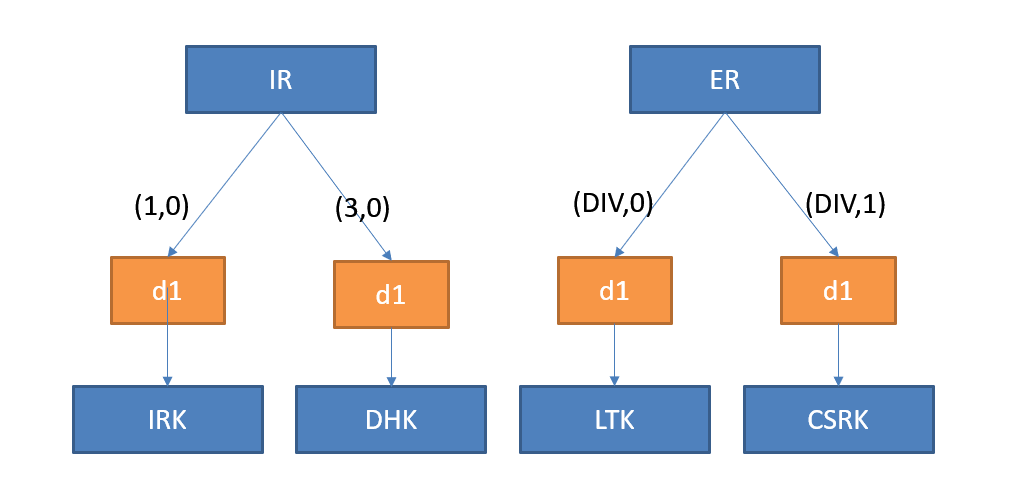
\includegraphics[width=0.85\linewidth]{./img/ble_keys} 

}

\caption{BLE 密钥层次结构}\label{fig:ch6-ble-keys}
\end{figure}

SM 涉及两个重要概念:

\begin{itemize}
\item
  \textbf{绑定}:在两个连接的设备之间交换秘密和身份信息以建立相互信赖关系。

  有的设备可能不支持绑定,因此规范定义了两种绑定模式:可绑定、不可绑定。
  建立绑定时需要使用\textbf{配对}流程交换秘密和身份信息。
\item
  \textbf{配对}:是一个用户层面的概念,需要用户输入识别码(passkey)。

  两种情况下会发生配对:1) 为了绑定;2) 用于认证未绑定的设备。
\end{itemize}

\hypertarget{ux4f7fux7528ux8bf4ux660e-6}{%
\section{使用说明}\label{ux4f7fux7528ux8bf4ux660e-6}}

\hypertarget{ux521dux59cbux5316}{%
\subsection{初始化}\label{ux521dux59cbux5316}}

\begin{enumerate}
\def\labelenumi{\arabic{enumi}.}
\item
  调用 \texttt{sm\_add\_event\_handler} 添加 SM 模块事件回调

\begin{Shaded}
\begin{Highlighting}[]
\DataTypeTok{void}\NormalTok{ sm_add_event_handler(}
  \CommentTok{// 回调函数}
\NormalTok{  btstack_packet_callback_registration_t * callback_handler);}
\end{Highlighting}
\end{Shaded}
\item
  调用 \texttt{sm\_config} 配置基础数据 ER、IR

\begin{Shaded}
\begin{Highlighting}[]
\DataTypeTok{void}\NormalTok{ sm_config(}
  \CommentTok{// 是否使能 SM(默认为不使能)}
  \DataTypeTok{uint8_t}\NormalTok{ enable,}
  \CommentTok{// 设备的 IO 能力}
\NormalTok{  io_capability_t io_capability,}
  \CommentTok{// 从角色时是否自动发送安全请求}
  \DataTypeTok{int}\NormalTok{   request_security,}
  \CommentTok{// 持久化数据}
  \DataTypeTok{const}\NormalTok{ sm_persistent_t *persistent);}
\end{Highlighting}
\end{Shaded}

  这里的 IO 能力 \texttt{io\_capability} 用于协商配对方法,跟设备的实际 IO 能力无关:

\begin{Shaded}
\begin{Highlighting}[]
\KeywordTok{typedef} \KeywordTok{enum}\NormalTok{ \{}
\NormalTok{  IO_CAPABILITY_UNINITIALIZED = -}\DecValTok{1}\NormalTok{,}
\NormalTok{  IO_CAPABILITY_DISPLAY_ONLY = }\DecValTok{0}\NormalTok{,   }\CommentTok{// 只支持显示}
\NormalTok{  IO_CAPABILITY_DISPLAY_YES_NO,     }\CommentTok{// 可显示,可输入 YES、NO}
\NormalTok{  IO_CAPABILITY_KEYBOARD_ONLY,      }\CommentTok{// 只能输入}
\NormalTok{  IO_CAPABILITY_NO_INPUT_NO_OUTPUT, }\CommentTok{// 无输入、输出能力}
\NormalTok{  IO_CAPABILITY_KEYBOARD_DISPLAY,   }\CommentTok{// 可显示,能输入}
\NormalTok{\} io_capability_t;}
\end{Highlighting}
\end{Shaded}

  这里的输入能力指可以输入 \(0-9\) 等 \(10\) 个数字,以及 YES、NO;显示能力是指可以显示 6 位十进制识别码(\(000000-999999\))\footnote{以及给予用户必要的提示的能力。}。

  持久化数据的定义如下:

\begin{Shaded}
\begin{Highlighting}[]
\KeywordTok{typedef} \KeywordTok{struct}\NormalTok{ sm_persistent}
\NormalTok{\{}
  \CommentTok{// ER 密钥}
\NormalTok{  sm_key_t        er;}
  \CommentTok{// IR 密钥}
\NormalTok{  sm_key_t        ir;}
  \CommentTok{// 身份地址}
\NormalTok{  bd_addr_t       identity_addr;}
  \CommentTok{// 身份地址类型(BD_ADDR_TYPE_LE_PUBLIC 或 BD_ADDR_TYPE_LE_RANDOM)}
\NormalTok{  bd_addr_type_t  identity_addr_type;}
\NormalTok{\} sm_persistent_t;}
\end{Highlighting}
\end{Shaded}
\item
  通过 \texttt{sm\_set\_authentication\_requirements} 设置认证需求

\begin{Shaded}
\begin{Highlighting}[]
\DataTypeTok{void}\NormalTok{ sm_set_authentication_requirements(}
  \CommentTok{// SM_AUTHREQ_... 的组合:是否绑定、是否需要 MITM 保护}
  \DataTypeTok{uint8_t}\NormalTok{ auth_req);}

\CommentTok{// 不可绑定}
\PreprocessorTok{#define SM_AUTHREQ_NO_BONDING       ...}
\CommentTok{// 可绑定}
\PreprocessorTok{#define SM_AUTHREQ_BONDING          ...}
\CommentTok{// 使能 MITM 保护}
\PreprocessorTok{#define SM_AUTHREQ_MITM_PROTECTION  ...}
\end{Highlighting}
\end{Shaded}
\end{enumerate}

\hypertarget{sm-ux4e8bux4ef6ux56deux8c03}{%
\subsection{SM 事件回调}\label{sm-ux4e8bux4ef6ux56deux8c03}}

SM 模块的事件回调函数将收到一系列事件,App 的主要工作就在于响应这些事件。

\begin{itemize}
\item
  \texttt{SM\_EVENT\_PRIVATE\_RANDOM\_ADDR\_UPDATE}

  SM 生成了一个新的私有随机地址。App 此时可以更新广播地址:

\begin{Shaded}
\begin{Highlighting}[]
\CommentTok{// 更新广播集 0 的随机地址}
\NormalTok{gap_set_adv_set_random_addr(}\DecValTok{0}\NormalTok{,}
\NormalTok{  sm_private_random_addr_update_get_address(packet));}
\end{Highlighting}
\end{Shaded}
\end{itemize}

与地址解析有关的 3 个事件:

\begin{itemize}
\item
  \texttt{SM\_EVENT\_IDENTITY\_RESOLVING\_STARTED}:开始解析某个地址

  使用以下 API 可读取正在解析的地址等信息:

  \begin{itemize}
  \tightlist
  \item
    \texttt{sm\_event\_identity\_resolving\_started\_get\_handle(packet)}:连接句柄
  \item
    \texttt{sm\_event\_identity\_resolving\_started\_get\_addr\_type(packet)}:正在解析的地址类型
  \item
    \texttt{sm\_event\_identity\_resolving\_started\_get\_address(packet,\ addr)}:正在解析的地址
  \end{itemize}
\item
  \texttt{SM\_EVENT\_IDENTITY\_RESOLVING\_FAILED}:解析失败

  使用以下 API 可读取解析失败的地址等信息:

  \begin{itemize}
  \tightlist
  \item
    \texttt{sm\_event\_identity\_resolving\_failed\_get\_handle(packet)}:连接句柄
  \item
    \texttt{sm\_event\_identity\_resolving\_failed\_get\_addr\_type(packet)}:正在解析的地址类型
  \item
    \texttt{sm\_event\_identity\_resolving\_failed\_get\_address(packet,\ addr)}:正在解析的地址
  \end{itemize}
\item
  \texttt{SM\_EVENT\_IDENTITY\_RESOLVING\_SUCCEEDED}:解析成功

  使用以下 API 可读取解析成功的地址等信息:

  \begin{itemize}
  \tightlist
  \item
    \texttt{sm\_event\_identity\_resolving\_succeeded\_get\_handle(packet)}:连接句柄
  \item
    \texttt{sm\_event\_identity\_resolving\_failed\_get\_addr\_type(packet)}:正在解析的地址类型
  \item
    \texttt{sm\_event\_identity\_resolving\_succeeded\_get\_address(packet,\ addr)}:正在解析的地址
  \item
    \texttt{sm\_event\_identity\_resolving\_succeeded\_get\_le\_device\_db\_index(packet)}:在\protect\hyperlink{ch98-le-dev-db}{设备数据库}里的序号
  \end{itemize}
\end{itemize}

与配对有关的 6 个事件:

\begin{itemize}
\item
  \texttt{SM\_EVENT\_JUST\_WORKS\_REQUEST}:JUST\_WORKS 请求,等待用户接收或拒绝

  调用 \texttt{sm\_just\_works\_confirm} 接受,\texttt{sm\_bonding\_decline} 拒绝。
\item
  \texttt{SM\_EVENT\_PASSKEY\_DISPLAY\_NUMBER}:显示识别码

  App 收到此事件后显示识别码,并提示用户在对端输入此识别码。
\item
  \texttt{SM\_EVENT\_PASSKEY\_DISPLAY\_CANCEL}:不要再显示识别码

  App 收到此事件后应该刷新显示,不再呈现识别码。
\item
  \texttt{SM\_EVENT\_PASSKEY\_INPUT\_NUMBER}:提示用户输入识别码

  App 收到此事件后提示用户输入识别码,然后调用 \texttt{sm\_passkey\_input} 把用户的输入传递到协议栈。
  调用 \texttt{sm\_bonding\_decline} 可中止配对。
\end{itemize}

SM 状态改变事件:

\begin{itemize}
\item
  \texttt{SM\_EVENT\_STATE\_CHANGED}

  这个事件指示 SM 总状态的变化。使用 \texttt{decode\_hci\_event} 将其解析为 \texttt{sm\_event\_state\_changed\_t}:

\begin{Shaded}
\begin{Highlighting}[]
\KeywordTok{typedef} \KeywordTok{struct}\NormalTok{ sm_event_state_changed \{}
  \CommentTok{// 连接句柄}
  \DataTypeTok{uint16_t}\NormalTok{ conn_handle;}
  \CommentTok{// 状态变化的原因}
  \DataTypeTok{uint8_t}\NormalTok{ reason;}
\NormalTok{\} sm_event_state_changed_t;}

\DataTypeTok{const}\NormalTok{ sm_event_state_changed_t *state_changed =}
\NormalTok{  decode_hci_event(packet, sm_event_state_changed_t);}
\end{Highlighting}
\end{Shaded}

  这里的 \texttt{reason} 即 SM 的几种\textbf{主要}状态:

\begin{Shaded}
\begin{Highlighting}[]
\KeywordTok{enum}\NormalTok{ sm_state_t}
\NormalTok{\{}
\NormalTok{  SM_STARTED,                 }\CommentTok{// SM 启动}
\NormalTok{  SM_FINAL_PAIRED,            }\CommentTok{// 已配对}
\NormalTok{  SM_FINAL_REESTABLISHED,     }\CommentTok{// 已重新建立}
\NormalTok{  SM_FINAL_FAIL_PROTOCOL,     }\CommentTok{// 协议流程错误}
\NormalTok{  SM_FINAL_FAIL_TIMEOUT,      }\CommentTok{// 超时}
\NormalTok{  SM_FINAL_FAIL_DISCONNECT,   }\CommentTok{// 连接断开}
\NormalTok{\};}
\end{Highlighting}
\end{Shaded}
\end{itemize}

\hypertarget{ux6bcfux4e2aux8fdeux63a5ux7684ux4e2aux6027ux5316ux8bbeux7f6e}{%
\subsection{每个连接的个性化设置}\label{ux6bcfux4e2aux8fdeux63a5ux7684ux4e2aux6027ux5316ux8bbeux7f6e}}

SM API 支持为每个连接进行个性化的设置:

\begin{Shaded}
\begin{Highlighting}[]
\DataTypeTok{void}\NormalTok{ sm_config_conn(}
  \CommentTok{// 连接句柄}
\NormalTok{  hci_con_handle_t con_handle,}
  \CommentTok{// IO 能力}
\NormalTok{  io_capability_t io_capability,}
  \CommentTok{// SM_AUTHREQ_... 的组合:是否绑定、是否需要 MITM 保护}
  \DataTypeTok{uint8_t}\NormalTok{ auth_req);}
\end{Highlighting}
\end{Shaded}

注意,这个 API 只允许在 HCI 事件 \texttt{HCI\_SUBEVENT\_LE\_ENHANCED\_CONNECTION\_COMPLETE} 的回调里调用。即使 SM 为禁用状态,
也可以使用这个 API 为单个连接使能 SM。

\hypertarget{ch-misc}{%
\chapter{杂项}\label{ch-misc}}

\hypertarget{ux63a5ux6536-cte}{%
\section{接收 CTE}\label{ux63a5ux6536-cte}}

共有四种 CTE 接收、发送方式\footnote{参考《Application Note: Direction Finding Solution》。}。
以 AoA 为例,各种方式的使用方法如下。

\hypertarget{ux57faux4e8eux8fdeux63a5ux7684-cte-ux63a5ux6536ux548cux53d1ux9001}{%
\subsection{基于连接的 CTE 接收和发送}\label{ux57faux4e8eux8fdeux63a5ux7684-cte-ux63a5ux6536ux548cux53d1ux9001}}

这种方式的使用可参考 SDK \emph{Central CTE} 和 \emph{Peripehral LED \& CTE}。

\hypertarget{ux53d1ux9001ux65b9}{%
\subsubsection{发送方}\label{ux53d1ux9001ux65b9}}

建立连接后:

\begin{enumerate}
\def\labelenumi{\arabic{enumi}.}
\item
  调用 \texttt{gap\_set\_connection\_cte\_tx\_param} 配置发送参数:

\begin{Shaded}
\begin{Highlighting}[]
\DataTypeTok{uint8_t}\NormalTok{ gap_set_connection_cte_tx_param(}
  \CommentTok{// 连接句柄}
  \DataTypeTok{const}\NormalTok{ hci_con_handle_t  conn_handle,}
  \CommentTok{// 允许发送的 CTE 类型组合}
  \DataTypeTok{const} \DataTypeTok{uint8_t}\NormalTok{           cte_types,}
  \CommentTok{// 用于 AoD 发送的天线切换模板的长度}
  \DataTypeTok{const} \DataTypeTok{uint8_t}\NormalTok{           switching_pattern_len,}
  \CommentTok{// 用于 AoD 发送的天线切换模板}
  \DataTypeTok{const} \DataTypeTok{uint8_t}\NormalTok{          *antenna_ids}
\NormalTok{);}
\end{Highlighting}
\end{Shaded}

  对于 AoA 模式,不需要配置天线切换模板,但是模板的长度必须至少为 \(2\):

\begin{Shaded}
\begin{Highlighting}[]
\NormalTok{gap_set_connection_cte_tx_param(}
\NormalTok{  con_handle, (}\DecValTok{1}\NormalTok{ << CTE_AOA), }\DecValTok{2}\NormalTok{, NULL);}
\end{Highlighting}
\end{Shaded}
\item
  调用 \texttt{gap\_set\_connection\_cte\_response\_enable} 使能 CTE 响应:

\begin{Shaded}
\begin{Highlighting}[]
\DataTypeTok{uint8_t}\NormalTok{ gap_set_connection_cte_response_enable(}
  \CommentTok{// 连接句柄}
  \DataTypeTok{const}\NormalTok{ hci_con_handle_t  conn_handle,}
  \CommentTok{// 是否使能}
  \DataTypeTok{const} \DataTypeTok{uint8_t}\NormalTok{           enable);}
\end{Highlighting}
\end{Shaded}
\end{enumerate}

\hypertarget{ux63a5ux6536ux65b9}{%
\subsubsection{接收方}\label{ux63a5ux6536ux65b9}}

使用 \texttt{ll\_set\_def\_antenna} 配置默认天线。建立连接后:

\begin{enumerate}
\def\labelenumi{\arabic{enumi}.}
\item
  调用 \texttt{gap\_set\_connection\_cte\_rx\_param} 配置接收参数:

\begin{Shaded}
\begin{Highlighting}[]
\DataTypeTok{uint8_t}\NormalTok{ gap_set_connection_cte_rx_param(}
  \CommentTok{// 连接句柄}
  \DataTypeTok{const}\NormalTok{ hci_con_handle_t  conn_handle,}
  \CommentTok{// 是否使能 CTE 采样}
  \DataTypeTok{const} \DataTypeTok{uint8_t}\NormalTok{           sampling_enable,}
  \CommentTok{// 时隙长度}
  \DataTypeTok{const}\NormalTok{ cte_slot_duration_type_t slot_durations,}
  \CommentTok{// 天线切换模板的长度}
  \DataTypeTok{const} \DataTypeTok{uint8_t}\NormalTok{           switching_pattern_len,}
  \CommentTok{// 天线切换模板}
  \DataTypeTok{const} \DataTypeTok{uint8_t}\NormalTok{          *antenna_ids);}
\end{Highlighting}
\end{Shaded}

  时隙长度共有两种:

\begin{Shaded}
\begin{Highlighting}[]
\KeywordTok{typedef} \KeywordTok{enum}
\NormalTok{\{}
\NormalTok{    CTE_SLOT_DURATION_1US = }\DecValTok{1}\NormalTok{,}
\NormalTok{    CTE_SLOT_DURATION_2US = }\DecValTok{2}
\NormalTok{\} cte_slot_duration_type_t;}
\end{Highlighting}
\end{Shaded}

  关于天线切换模板的更多信息请参考《Application Note: Direction Finding Solution》。
\item
  调用 \texttt{gap\_set\_connection\_cte\_request\_enable} 开始发送 CTE 请求

  连接模式的 CTE 为按需发送:一方发送一次 CTE 请求,对方就响应一次。

\begin{Shaded}
\begin{Highlighting}[]
\DataTypeTok{uint8_t}\NormalTok{ gap_set_connection_cte_request_enable(}
  \CommentTok{// 连接句柄}
  \DataTypeTok{const}\NormalTok{ hci_con_handle_t  conn_handle,}
  \CommentTok{// 是否使能}
  \DataTypeTok{const} \DataTypeTok{uint8_t}\NormalTok{           enable,}
  \CommentTok{// 发送 CTE 请求的间隔}
  \DataTypeTok{const} \DataTypeTok{uint16_t}\NormalTok{          requested_cte_interval,}
  \CommentTok{// 请求的 CTE 的长度(范围 2~20,单位 8μs)}
  \DataTypeTok{const} \DataTypeTok{uint8_t}\NormalTok{           requested_cte_length,}
  \CommentTok{// 请求的 CTE 的类型}
  \DataTypeTok{const}\NormalTok{ cte_type_t        requested_cte_type);}
\end{Highlighting}
\end{Shaded}

  \texttt{requested\_cte\_interval} 表示每 \texttt{requested\_cte\_interval} 个连接间隔发送一次 CTE 请求, \(0\) 表示只发送一次。
  对于 AoA,\texttt{requested\_cte\_type} 为 \texttt{CTE\_AOA}。
\item
  响应 \texttt{HCI\_SUBEVENT\_LE\_CONNECTION\_IQ\_REPORT} 事件

  使用 \texttt{decode\_hci\_le\_meta\_event} 解析事件内容:

\begin{Shaded}
\begin{Highlighting}[]
\DataTypeTok{const}\NormalTok{ le_meta_conn_iq_report_t *rpt =}
\NormalTok{  decode_hci_le_meta_event(packet, le_meta_conn_iq_report_t);}
\end{Highlighting}
\end{Shaded}

  如果 CTE 请求失败(未收到响应),则会收到 \texttt{HCI\_SUBEVENT\_LE\_CTE\_REQ\_FAILED} 事件。
\end{enumerate}

\hypertarget{misc-cte-periodic-adv}{%
\subsection{基于周期广播的 CTE 接收和发送}\label{misc-cte-periodic-adv}}

这种方式的使用可参考 SDK \emph{Periodic Advertiser} 和 \emph{Periodic Scanner}。

\hypertarget{ux53d1ux9001ux65b9-1}{%
\subsubsection{发送方}\label{ux53d1ux9001ux65b9-1}}

使能周期广播后,

\begin{enumerate}
\def\labelenumi{\arabic{enumi}.}
\item
  调用 \texttt{gap\_set\_connectionless\_cte\_tx\_param} 配置 CTE 发送参数

\begin{Shaded}
\begin{Highlighting}[]
\DataTypeTok{uint8_t}\NormalTok{ gap_set_connectionless_cte_tx_param(}
  \CommentTok{// 广播句柄}
  \DataTypeTok{const} \DataTypeTok{uint8_t}\NormalTok{       adv_handle,}
  \CommentTok{// CTE 长度(范围 2~20,单位 8μs)}
  \DataTypeTok{const} \DataTypeTok{uint8_t}\NormalTok{       cte_len,}
  \CommentTok{// CTE 类型(对于 AoA,即 CTE_AOA)}
  \DataTypeTok{const}\NormalTok{ cte_type_t    cte_type,}
  \CommentTok{// 一个周期广播里 CTE 发送次数}
  \DataTypeTok{const} \DataTypeTok{uint8_t}\NormalTok{       cte_count,}
  \CommentTok{// 用于 AoD 发送的天线切换模板的长度}
  \DataTypeTok{const} \DataTypeTok{uint8_t}\NormalTok{       switching_pattern_len,}
  \CommentTok{// 用于 AoD 发送的天线切换模板}
  \DataTypeTok{const} \DataTypeTok{uint8_t}\NormalTok{      *antenna_ids);}
\end{Highlighting}
\end{Shaded}
\item
  调用 \texttt{gap\_set\_connectionless\_cte\_tx\_enable} 使能 CTE 发送

\begin{Shaded}
\begin{Highlighting}[]
\DataTypeTok{uint8_t}\NormalTok{ gap_set_connectionless_cte_tx_enable(}
  \CommentTok{// 广播句柄}
  \DataTypeTok{const} \DataTypeTok{uint8_t}\NormalTok{       adv_handle,}
  \CommentTok{// 是否使能}
  \DataTypeTok{const} \DataTypeTok{uint8_t}\NormalTok{       cte_enable);}
\end{Highlighting}
\end{Shaded}

  \hypertarget{ux63a5ux6536ux65b9-1}{%
  \subsubsection{接收方}\label{ux63a5ux6536ux65b9-1}}
\end{enumerate}

与周期广播建立同步后,调用 \texttt{gap\_set\_connectionless\_iq\_sampling\_enable} 启动 CTE 接收。

\begin{Shaded}
\begin{Highlighting}[]
\DataTypeTok{uint8_t}\NormalTok{ gap_set_connectionless_iq_sampling_enable(}
  \CommentTok{// 同步句柄}
  \DataTypeTok{const} \DataTypeTok{uint16_t}\NormalTok{      sync_handle,}
  \CommentTok{// 是否使能采样}
  \DataTypeTok{const} \DataTypeTok{uint8_t}\NormalTok{       sampling_enable,}
  \CommentTok{// 时隙长度}
  \DataTypeTok{const}\NormalTok{ cte_slot_duration_type_t slot_durations,}
  \CommentTok{// 每个周期广播间隔内最多接收多少个 CTE}
  \DataTypeTok{const} \DataTypeTok{uint8_t}\NormalTok{       max_sampled_ctes,}
  \CommentTok{// 天线切换模板长度}
  \DataTypeTok{const} \DataTypeTok{uint8_t}\NormalTok{       switching_pattern_len,}
  \CommentTok{// 天线切换模板}
  \DataTypeTok{const} \DataTypeTok{uint8_t}\NormalTok{      *antenna_ids);}
\end{Highlighting}
\end{Shaded}

此后就可以周期性收到 \texttt{HCI\_SUBEVENT\_LE\_CONNECTIONLESS\_IQ\_REPORT} 事件,利用 \texttt{decode\_hci\_le\_meta\_event}
解析事件内容:

\begin{Shaded}
\begin{Highlighting}[]
\DataTypeTok{const}\NormalTok{ le_meta_connless_iq_report_t *rpt =}
\NormalTok{  decode_hci_le_meta_event(packet, le_meta_connless_iq_report_t);}
\end{Highlighting}
\end{Shaded}

\hypertarget{ux57faux4e8eux79c1ux6709ux65b9ux5f0f-1-ux7684-cte-ux63a5ux6536ux548cux53d1ux9001}{%
\subsection{基于私有方式 \#1 的 CTE 接收和发送}\label{ux57faux4e8eux79c1ux6709ux65b9ux5f0f-1-ux7684-cte-ux63a5ux6536ux548cux53d1ux9001}}

这种方式最为灵活,需要配置的参数也最多,可参考 SDK \emph{Ext. Raw Packet Tx/Rx}。

\hypertarget{ux57faux4e8eux79c1ux6709ux65b9ux5f0f-2-ux7684-cte-ux63a5ux6536ux548cux53d1ux9001}{%
\subsection{基于私有方式 \#2 的 CTE 接收和发送}\label{ux57faux4e8eux79c1ux6709ux65b9ux5f0f-2-ux7684-cte-ux63a5ux6536ux548cux53d1ux9001}}

这种方式的使用可参考 SDK \emph{Central CTE} 和 \emph{Peripehral LED \& CTE}。

\hypertarget{ux53d1ux9001ux65b9-2}{%
\subsubsection{发送方}\label{ux53d1ux9001ux65b9-2}}

配置一个扩展广播集,属性设置为不可连接、不可扫描。待广播集使能后,调用 \texttt{ll\_attach\_cte\_to\_adv\_set}\footnote{参考《Controller API Reference》。}
为扩展广播附加 CTE。

\hypertarget{ux63a5ux6536ux65b9-2}{%
\subsubsection{接收方}\label{ux63a5ux6536ux65b9-2}}

启动扫描之后,调用 \texttt{ll\_scanner\_enable\_iq\_sampling}\footnote{参考《Controller API Reference》。} 使能 CTE 采样。
之后,通过 \texttt{HCI\_SUBEVENT\_LE\_VENDOR\_PRO\_CONNECTIONLESS\_IQ\_REPORT} 事件获得 CTE 报告。

\hypertarget{ux517cux5bb9ux6027}{%
\section{兼容性}\label{ux517cux5bb9ux6027}}

\hypertarget{data-length-ux4e0e-mtu}{%
\subsection{Data Length 与 MTU}\label{data-length-ux4e0e-mtu}}

低功耗蓝牙进入连接模式后,各层分别协商通信中数据包的大小,对于 ATT 层,由 MTU EXCHANGE 流程实现;对于链路层,由 DATA LENGTH 更新流程实现。

按照规范,进入连接模式后,DATA LENGTH 更新流程可以由主或从设备在任何时刻发起。这导致了一个问题:某些芯片无法处理对方设备``随时''发起的
DATA LENGTH 更新流程\footnote{\url{https://ingchips.github.io/blog/2021-06-02-sdk-6/\#\%E5\%85\%BC\%E5\%AE\%B9\%E6\%80\%A7}}。
为了更新地兼容不同的芯片,协议栈定义了两个配置项:

\begin{Shaded}
\begin{Highlighting}[]
\KeywordTok{enum}\NormalTok{ btstack_config_item \{}
\NormalTok{    STACK_ATT_SERVER_ENABLE_AUTO_DATA_LEN_REQ = }\DecValTok{1}\NormalTok{,}
\NormalTok{    STACK_GATT_CLIENT_DISABLE_AUTO_DATA_LEN_REQ = }\DecValTok{2}\NormalTok{,}
    \CommentTok{//...}
\NormalTok{\};}
\end{Highlighting}
\end{Shaded}

这两个配置分别控制 GATT Server、Client 在 MTU EXCHANGE 时是否自动发起 DATA LENGTH 更新流程。默认情况下,Servier 不会自动发起更新流程,
而 Client 会自动发起。

通过 \texttt{btstack\_config} 配置:

\begin{Shaded}
\begin{Highlighting}[]
\DataTypeTok{void}\NormalTok{ btstack_config(}
  \CommentTok{// btstack_config_item 的比特组合}
  \DataTypeTok{uint32_t}\NormalTok{ flags);}
\end{Highlighting}
\end{Shaded}

\hypertarget{api-ux8fd4ux56deux503c}{%
\section{API 返回值}\label{api-ux8fd4ux56deux503c}}

绝大多数协议栈 API 都带有 \texttt{uint8\_t} 型的返回值,\(0\) 为成功,非 \(0\) 为错误。开发者需要关注这些返回值。

几个例子:

\begin{itemize}
\item
  \texttt{att\_server\_notify} 的返回值:

  \begin{itemize}
  \tightlist
  \item
    \(0\):成功
  \item
    \texttt{BTSTACK\_LE\_CHANNEL\_NOT\_EXIST}:连接不存在(连接句柄参数错误?)
  \item
    \texttt{BTSTACK\_ACL\_BUFFERS\_FULL}:内存已满
  \end{itemize}
\item
  \texttt{gap\_set\_ext\_adv\_para} 的返回值:

  \begin{itemize}
  \tightlist
  \item
    \(0\):成功
  \item
    \texttt{BTSTACK\_MEMORY\_ALLOC\_FAILED}:内存已满
  \end{itemize}
\end{itemize}

\hypertarget{ux952eux503cux5b58ux50a8}{%
\section{键值存储}\label{ux952eux503cux5b58ux50a8}}

协议包含了一个简单的键值存储模块(\emph{kv\_storage}),其键(\emph{key}) 为 \texttt{uint8\_t},值(\emph{value}) 为长度不超过 \texttt{KV\_VALUE\_MAX\_LEN}
的数组。

开发者可以在 App 里使用这个模块,\emph{key} 的取值范围应该在 \texttt{KV\_USER\_KEY\_START} 和 \texttt{KV\_USER\_KEY\_END} 之间。需要注意以下几点:

\begin{enumerate}
\def\labelenumi{\arabic{enumi}.}
\tightlist
\item
  该模块查找一个 \emph{key} 的时间复杂度为 \(\mathcal{O}(n)\);
\item
  该模块不是线程安全的。
\end{enumerate}

这个模块本身没有数据持久化。持久化需要开发者通过 \texttt{kv\_init} 提供回调来实现:

\begin{Shaded}
\begin{Highlighting}[]
\DataTypeTok{void}\NormalTok{ kv_init(}
  \CommentTok{// 用来保存数据的回调}
\NormalTok{  f_kv_write_to_nvm f_write,}
  \CommentTok{// 用来读取(恢复)数据的回调}
\NormalTok{  f_kv_read_from_nvm f_read);}
\end{Highlighting}
\end{Shaded}

当键值存储模块初始化时,会调用 \texttt{f\_read} 恢复之前的数据状态;当存储里的数据更新后,键值存储模块会自动调用 \texttt{f\_write} 回调。
考虑到 Flash 不宜频繁擦写,键值存储模块通过定时器超时来触发写入。每当数据更新时,复位定时器。整个储存的总大小为
\texttt{DB\_CAPACITY\_SIZE}。

这个存储模块的增、删、改、查等接口如下。

\begin{itemize}
\item
  增/改:\texttt{kv\_put}

\begin{Shaded}
\begin{Highlighting}[]
\CommentTok{// 如果 key 不存在,为“增”;如果 key 存在,为“改”}
\DataTypeTok{int}\NormalTok{ kv_put(}
  \DataTypeTok{const}\NormalTok{ kvkey_t key,}
  \CommentTok{// 值}
  \DataTypeTok{const} \DataTypeTok{uint8_t}\NormalTok{ *data,}
  \CommentTok{// 值的长度}
  \DataTypeTok{int16_t}\NormalTok{ len);}
\end{Highlighting}
\end{Shaded}
\item
  删:\texttt{kv\_remove}

\begin{Shaded}
\begin{Highlighting}[]
\DataTypeTok{void}\NormalTok{ kv_remove(}
  \CommentTok{// 键}
  \DataTypeTok{const}\NormalTok{ kvkey_t key)}
\end{Highlighting}
\end{Shaded}
\item
  查:\texttt{kv\_get}

\begin{Shaded}
\begin{Highlighting}[]
\CommentTok{// 返回:指向值的指针}
\DataTypeTok{uint8_t}\NormalTok{ *kv_get(}
  \CommentTok{// 键}
  \DataTypeTok{const}\NormalTok{ kvkey_t key,}
  \CommentTok{// 输出:值的长度}
  \DataTypeTok{int16_t}\NormalTok{ *len);}
\end{Highlighting}
\end{Shaded}

  这个 API 返回的指针直接指向模块内值的存储空间,允许开发者在不改变值的长度的前提下修改其的内容。
  修改之后需要调用 \texttt{kv\_value\_modified} 告知存储模块。
\item
  遍历:\texttt{kv\_visit}

\begin{Shaded}
\begin{Highlighting}[]
\DataTypeTok{void}\NormalTok{ kv_visit(}
  \CommentTok{// 访问者回调}
\NormalTok{  f_kv_visitor visitor,}
  \CommentTok{// 传递给回调的用户参数}
  \DataTypeTok{void}\NormalTok{ *user_data);}
\end{Highlighting}
\end{Shaded}

  使用这个 API 可以遍历存储内所有的键值对。
\end{itemize}

\hypertarget{ch98-le-dev-db}{%
\section{设备数据库}\label{ch98-le-dev-db}}

设备数据库模块(\emph{le\_device\_db})负责存储、管理设备的绑定信息。这个模块是基于键值存储模块实现的。
删、查等接口如下。

\begin{itemize}
\item
  查:\texttt{le\_device\_db\_find}

\begin{Shaded}
\begin{Highlighting}[]
\NormalTok{le_device_memory_db_t *le_device_db_find(}
  \CommentTok{// 待查设备的地址类型}
  \DataTypeTok{const} \DataTypeTok{int}\NormalTok{ addr_type,}
  \CommentTok{// 待查设备的地址}
  \DataTypeTok{const}\NormalTok{ bd_addr_t addr,}
  \CommentTok{// 输出:在数据库里的序号}
  \DataTypeTok{int}\NormalTok{ *index);}
\end{Highlighting}
\end{Shaded}
\item
  删

  直接按地址删除:

\begin{Shaded}
\begin{Highlighting}[]
\DataTypeTok{void}\NormalTok{ le_device_db_remove(}
  \CommentTok{// 待删设备的地址类型}
  \DataTypeTok{const} \DataTypeTok{int}\NormalTok{ addr_type,}
  \CommentTok{// 待删设备的地址}
  \DataTypeTok{const}\NormalTok{ bd_addr_t addr);}
\end{Highlighting}
\end{Shaded}

  根据在数据库里的编号删除:

\begin{Shaded}
\begin{Highlighting}[]
\DataTypeTok{void}\NormalTok{ le_device_db_remove_key(}
  \CommentTok{// 待删设备在数据库里的编号}
  \DataTypeTok{int}\NormalTok{ index);}
\end{Highlighting}
\end{Shaded}
\item
  遍历

  这个模块支持迭代器遍历:

\begin{Shaded}
\begin{Highlighting}[]
\NormalTok{le_device_memory_db_iter_t iter;}
\NormalTok{le_device_db_iter_init(&iter);}
\ControlFlowTok{while}\NormalTok{ (le_device_db_iter_next(&iter))}
\NormalTok{\{}
\NormalTok{    le_device_memory_db_t *cur = le_device_db_iter_cur(&iter);}
    \CommentTok{// ...}
\NormalTok{\}}
\end{Highlighting}
\end{Shaded}
\end{itemize}

\hypertarget{ch-cap}{%
\chapter{协议栈能力}\label{ch-cap}}

对于不同的软件包、不同的芯片系列,协议栈能力不同,汇总\footnote{依据 SDK v8.1.0。}于表 \ref{tab:ch99-typical-stack-cap} 和 表 \ref{tab:ch99-mass-conn-stack-cap}。

\begin{longtable}[]{@{}lccccc@{}}
\caption{\label{tab:ch99-typical-stack-cap} \{\emph{typical}, \emph{extension},\emph{exp}\} 软件包协议栈能力}\tabularnewline
\toprule
系列 & 广播集数目 & 连接数目 & 白名单容量 & CTE & 最大 MTU\tabularnewline
\midrule
\endfirsthead
\toprule
系列 & 广播集数目 & 连接数目 & 白名单容量 & CTE & 最大 MTU\tabularnewline
\midrule
\endhead
ING9188X & \(8\) & \(8\) & \(16\) & \(\checkmark\) & \(247\)\tabularnewline
ING9187X & \(8\) & \(8\) & \(16\) & & \(247\)\tabularnewline
ING9186X & \(4\) & \(4\) & \(8\) & \(\checkmark\) & \(247\)\tabularnewline
ING9185X & \(4\) & \(4\) & \(8\) & & \(247\)\tabularnewline
ING916XX & \(4\) & \(4\) & \(8\) & \(\checkmark\) & \(247\)\tabularnewline
\bottomrule
\end{longtable}

\begin{longtable}[]{@{}lccccc@{}}
\caption{\label{tab:ch99-mass-conn-stack-cap} \{\emph{mass\_conn}\} 软件包协议栈能力}\tabularnewline
\toprule
系列 & 广播集数目 & 连接数目 & 白名单容量 & CTE & 最大 MTU\tabularnewline
\midrule
\endfirsthead
\toprule
系列 & 广播集数目 & 连接数目 & 白名单容量 & CTE & 最大 MTU\tabularnewline
\midrule
\endhead
ING9188X & \(8\) & \(26\) & \(24\) & \(\checkmark\) & \(247\)\tabularnewline
ING9187X & \(8\) & \(26\) & \(24\) & & \(247\)\tabularnewline
\bottomrule
\end{longtable}

  \bibliography{book.bib,packages.bib}

\backmatter
\printindex

\end{document}
